\PassOptionsToPackage{unicode=true}{hyperref} % options for packages loaded elsewhere
\PassOptionsToPackage{hyphens}{url}
%
\documentclass[]{book}
\usepackage{lmodern}
\usepackage{amssymb,amsmath}
\usepackage{ifxetex,ifluatex}
\usepackage{fixltx2e} % provides \textsubscript
\ifnum 0\ifxetex 1\fi\ifluatex 1\fi=0 % if pdftex
  \usepackage[T1]{fontenc}
  \usepackage[utf8]{inputenc}
  \usepackage{textcomp} % provides euro and other symbols
\else % if luatex or xelatex
  \usepackage{unicode-math}
  \defaultfontfeatures{Ligatures=TeX,Scale=MatchLowercase}
\fi
% use upquote if available, for straight quotes in verbatim environments
\IfFileExists{upquote.sty}{\usepackage{upquote}}{}
% use microtype if available
\IfFileExists{microtype.sty}{%
\usepackage[]{microtype}
\UseMicrotypeSet[protrusion]{basicmath} % disable protrusion for tt fonts
}{}
\IfFileExists{parskip.sty}{%
\usepackage{parskip}
}{% else
\setlength{\parindent}{0pt}
\setlength{\parskip}{6pt plus 2pt minus 1pt}
}
\usepackage{hyperref}
\hypersetup{
            pdftitle={Assessing the causal association of mtDNAcn with Alzheimer's disease},
            pdfauthor={Dr.~Shea Andrews},
            pdfborder={0 0 0},
            breaklinks=true}
\urlstyle{same}  % don't use monospace font for urls
\usepackage{color}
\usepackage{fancyvrb}
\newcommand{\VerbBar}{|}
\newcommand{\VERB}{\Verb[commandchars=\\\{\}]}
\DefineVerbatimEnvironment{Highlighting}{Verbatim}{commandchars=\\\{\}}
% Add ',fontsize=\small' for more characters per line
\usepackage{framed}
\definecolor{shadecolor}{RGB}{248,248,248}
\newenvironment{Shaded}{\begin{snugshade}}{\end{snugshade}}
\newcommand{\AlertTok}[1]{\textcolor[rgb]{0.94,0.16,0.16}{#1}}
\newcommand{\AnnotationTok}[1]{\textcolor[rgb]{0.56,0.35,0.01}{\textbf{\textit{#1}}}}
\newcommand{\AttributeTok}[1]{\textcolor[rgb]{0.77,0.63,0.00}{#1}}
\newcommand{\BaseNTok}[1]{\textcolor[rgb]{0.00,0.00,0.81}{#1}}
\newcommand{\BuiltInTok}[1]{#1}
\newcommand{\CharTok}[1]{\textcolor[rgb]{0.31,0.60,0.02}{#1}}
\newcommand{\CommentTok}[1]{\textcolor[rgb]{0.56,0.35,0.01}{\textit{#1}}}
\newcommand{\CommentVarTok}[1]{\textcolor[rgb]{0.56,0.35,0.01}{\textbf{\textit{#1}}}}
\newcommand{\ConstantTok}[1]{\textcolor[rgb]{0.00,0.00,0.00}{#1}}
\newcommand{\ControlFlowTok}[1]{\textcolor[rgb]{0.13,0.29,0.53}{\textbf{#1}}}
\newcommand{\DataTypeTok}[1]{\textcolor[rgb]{0.13,0.29,0.53}{#1}}
\newcommand{\DecValTok}[1]{\textcolor[rgb]{0.00,0.00,0.81}{#1}}
\newcommand{\DocumentationTok}[1]{\textcolor[rgb]{0.56,0.35,0.01}{\textbf{\textit{#1}}}}
\newcommand{\ErrorTok}[1]{\textcolor[rgb]{0.64,0.00,0.00}{\textbf{#1}}}
\newcommand{\ExtensionTok}[1]{#1}
\newcommand{\FloatTok}[1]{\textcolor[rgb]{0.00,0.00,0.81}{#1}}
\newcommand{\FunctionTok}[1]{\textcolor[rgb]{0.00,0.00,0.00}{#1}}
\newcommand{\ImportTok}[1]{#1}
\newcommand{\InformationTok}[1]{\textcolor[rgb]{0.56,0.35,0.01}{\textbf{\textit{#1}}}}
\newcommand{\KeywordTok}[1]{\textcolor[rgb]{0.13,0.29,0.53}{\textbf{#1}}}
\newcommand{\NormalTok}[1]{#1}
\newcommand{\OperatorTok}[1]{\textcolor[rgb]{0.81,0.36,0.00}{\textbf{#1}}}
\newcommand{\OtherTok}[1]{\textcolor[rgb]{0.56,0.35,0.01}{#1}}
\newcommand{\PreprocessorTok}[1]{\textcolor[rgb]{0.56,0.35,0.01}{\textit{#1}}}
\newcommand{\RegionMarkerTok}[1]{#1}
\newcommand{\SpecialCharTok}[1]{\textcolor[rgb]{0.00,0.00,0.00}{#1}}
\newcommand{\SpecialStringTok}[1]{\textcolor[rgb]{0.31,0.60,0.02}{#1}}
\newcommand{\StringTok}[1]{\textcolor[rgb]{0.31,0.60,0.02}{#1}}
\newcommand{\VariableTok}[1]{\textcolor[rgb]{0.00,0.00,0.00}{#1}}
\newcommand{\VerbatimStringTok}[1]{\textcolor[rgb]{0.31,0.60,0.02}{#1}}
\newcommand{\WarningTok}[1]{\textcolor[rgb]{0.56,0.35,0.01}{\textbf{\textit{#1}}}}
\usepackage{longtable,booktabs}
% Fix footnotes in tables (requires footnote package)
\IfFileExists{footnote.sty}{\usepackage{footnote}\makesavenoteenv{longtable}}{}
\usepackage{graphicx,grffile}
\makeatletter
\def\maxwidth{\ifdim\Gin@nat@width>\linewidth\linewidth\else\Gin@nat@width\fi}
\def\maxheight{\ifdim\Gin@nat@height>\textheight\textheight\else\Gin@nat@height\fi}
\makeatother
% Scale images if necessary, so that they will not overflow the page
% margins by default, and it is still possible to overwrite the defaults
% using explicit options in \includegraphics[width, height, ...]{}
\setkeys{Gin}{width=\maxwidth,height=\maxheight,keepaspectratio}
\setlength{\emergencystretch}{3em}  % prevent overfull lines
\providecommand{\tightlist}{%
  \setlength{\itemsep}{0pt}\setlength{\parskip}{0pt}}
\setcounter{secnumdepth}{5}
% Redefines (sub)paragraphs to behave more like sections
\ifx\paragraph\undefined\else
\let\oldparagraph\paragraph
\renewcommand{\paragraph}[1]{\oldparagraph{#1}\mbox{}}
\fi
\ifx\subparagraph\undefined\else
\let\oldsubparagraph\subparagraph
\renewcommand{\subparagraph}[1]{\oldsubparagraph{#1}\mbox{}}
\fi

% set default figure placement to htbp
\makeatletter
\def\fps@figure{htbp}
\makeatother

\usepackage{booktabs}
\usepackage[]{natbib}
\bibliographystyle{apalike}

\title{Assessing the causal association of mtDNAcn with Alzheimer's disease}
\author{Dr.~Shea Andrews}
\date{28 May, 2020}

\begin{document}
\maketitle

{
\setcounter{tocdepth}{1}
\tableofcontents
}
\hypertarget{abstract}{%
\chapter*{Abstract}\label{abstract}}
\addcontentsline{toc}{chapter}{Abstract}

Increasing evidence has implicated mitochondrial dysfunction in Alzheimer's Disease (AD). As AD features altered mitochondrial function, this suggests that therapeutics strategies aimed at preventing declines in mitochondrial function may modify the disease course in AD. However, it is unclear whether mitochondrial dysfunction causes, mediates, or is a by-product of AD pathogenesis. As mitochondria contain their own DNA outside of the nuclear genome, with every cell having between 100-10,000 copies of mitochondrial DNA, mitochondrial DNA copy number (mtDNA-CN) can be used as a surrogate measure of mitochondrial function. The overall objective of this research program is to evaluate whether mitochondrial dysfunction plays a causal role in AD pathogenesis. Our central hypothesis is that lower mtDNA-CN -- indicative of mitochondrial dysfunction -- will be associated with increased risk of AD. This study will disentangle the causal role of mitochondrial dysfunction in AD using traditional epidemiological approaches, polygenic risk scoring (PRS) and Mendelian randomization (MR). PRS are a measure of an individual's genetic propensity to a trait and can be used to evaluate the genetic overlap between two traits by testing whether the PRS of one trait predicts another trait, while MR uses genetic variants to estimate the causal effect of risk factors on disease outcomes. In the first aim, we will calculate in mtDNA-CN in AD cases and controls and evaluate the association between mtDNA-CN and AD. In the second aim, we will construct a PRS for mtDNA-CN and determine if genetically predicted mtDNA-CN is associated with AD outcomes. In the final aim, we will use MR to evaluate the causal effect of mtDNA-CN on AD outcomes and the causal effect of AD on mtDNA-CN. By establishing if mitochondrial dysfunction has a causal role in AD pathogenesis, this study will provide evidence regarding the utility of mitochondrial therapeutic strategies in AD.

\hypertarget{intro}{%
\chapter{Introduction}\label{intro}}

\hypertarget{neuropathological-confirmed-ad}{%
\section{Neuropathological Confirmed AD}\label{neuropathological-confirmed-ad}}

There is consensus to disentangle the clinicopathologic term ``Alzheimer's disease'' from AD neuropathologic change. The former refers to clinical signs and symptoms of cognitive and behavioral changes that are typical for patients who have substantial AD neuropathologic change,and is the focus of recent NIA--AA-sponsored consensus re-ports on three defined stages in a clinical continuum that includes preclinical, mild cognitive impairment, anddementia. The latter refers to the presence and extentof neuropathologic changes of AD observed at autopsy, re-gardless of the clinical setting.

\hypertarget{cerad-criteria---1991}{%
\subsection{CERAD Criteria - 1991}\label{cerad-criteria---1991}}

Protocol provides neuropathologic definitions of such terms as ``definite Alzheimer's disease'' (AD), ``probable AD,'' ``possible AD,'' and ``normal brain'' to indicate levels of diagnostic certainty (\citet{Mirra479}). The CERAD Neuritic Plaque score forms the basis of later neuropathological difinitions.

Sections are tacken from:

\begin{itemize}
\tightlist
\item
  \href{https://en.wikipedia.org/wiki/Middle_frontal_gyrus}{middle frontal gyrus}
\item
  \href{https://en.wikipedia.org/wiki/Superior_temporal_gyrus}{superior} and \href{https://en.wikipedia.org/wiki/Middle_temporal_gyrus}{middle} temporal gyri
\item
  \href{https://en.wikipedia.org/wiki/Inferior_parietal_lobule}{inferior parietal lobule}
\item
  \href{https://en.wikipedia.org/wiki/Hippocampus}{hippocampus} and \href{https://en.wikipedia.org/wiki/Entorhinal_cortex}{entorhinal cortex}
\item
  \href{https://en.wikipedia.org/wiki/Midbrain}{midbrain}
\end{itemize}

And scored as a semiquantitative measurment:

\begin{itemize}
\tightlist
\item
  Absent
\item
  Sparese
\item
  Moderate
\item
  Frequent
\end{itemize}

An age-related plaque score is then determined by combining the age of the patient at death and the semiquantitative measure of plaques in the \emph{most severely affected region of the neocortex}. This score is then intergrated with with clinical information the presence or absence of dementia.

\hypertarget{nia-reagan-criteria---1997}{%
\subsection{NIA-Reagan Criteria - 1997}\label{nia-reagan-criteria---1997}}

The modified NIA-Reagan diagnosis of Alzheimer's disease is based on consensus recommendations for postmortem diagnosis of Alzheimer's disease. The criteria rely on both neurofibrillary tangles (Braak) and neuritic plaques (CERAD). See \href{https://doi.org/10.1016/S0197-4580(97)00057-2}{NIA Working group consensus 1997} and corresponding editorial by \href{https://doi.org/10.1097/00005072-199710000-00002}{Hyman et al 1997}. Traditionaly, the criteria require a history of dementia, insofar as they were designed to help address the question of whether AD was the underlying cause of a patient's dementia.

\begin{itemize}
\tightlist
\item
  CERAD score is a semiquantitative measure of neuritic plaques

  \begin{itemize}
  \tightlist
  \item
    No neuritic plaques (C0)
  \item
    Sparse/infrequent neuritic plaques (C1)
  \item
    Moderate neuritic plaques (C2)
  \item
    Frequent neuritic plaques (C3)
  \end{itemize}
\item
  Braak Stage is a semiquantitative measure of severity of neurofibrillary tangle (NFT) pathology.

  \begin{itemize}
  \tightlist
  \item
    no NFTs (B0)
  \item
    stages I/II, with NFTs predominantly in en-torhinal cortex and closely related areas (B1)
  \item
    stages III/IV, withNFTs more abundant in hippocampus and amygdala whileextending slightly into association cortex (B2)
  \item
    stages V/VI,with NFTs widely distributed throughout the neocortex (B3)
  \end{itemize}
\end{itemize}

\begin{longtable}[]{@{}lllll@{}}
\toprule
CERAD / Braak & 0 & I/II & III/IV & V/VI\tabularnewline
\midrule
\endhead
None & \textbf{Normal} & - & - & -\tabularnewline
Sparse & - & \textbf{Low} & - & -\tabularnewline
Moderate & - & - & \textbf{Intermediate} & -\tabularnewline
Frequent & - & - & - & \textbf{High}\tabularnewline
\bottomrule
\end{longtable}

\hypertarget{nia-aa-criteria---2012}{%
\subsection{NIA-AA Criteria - 2012}\label{nia-aa-criteria---2012}}

The NIA-AA criteria updated and revised the 1997 NIA-Reagan criteria to recognize the pre-clinical stage of AD, enhance the assessment of AD to include amyloid accumulation as well as neurofibrillary change and neuritic plaques. Hyman et al 2012. The criteria relies on an `ABC' score for AD neuropathologic change that incorporates histopathologic assessments of amyloid β deposits (A - Thal phase), staging of neurofibrillary tangles (B - CERAD), and scoring of neuritic plaques (C - Braak Stage). See \href{https://doi.org/10.1016/j.jalz.2011.10.007}{Hyman et al 2012} for guidlines and \href{https://doi.org/10.1007/s00401-011-0910-3}{Montine et al 2012} for a practial guide.

\begin{itemize}
\tightlist
\item
  Thal Phase is a semiquantitiative measure of the distribution of AB

  \begin{itemize}
  \tightlist
  \item
    phase 0 or no amyloid
  \item
    phase 1 or isocortical
  \item
    phase 2 or limbic
  \item
    phase 3 or basal ganglia
  \item
    phase 4 or basal forebrain and midbrain
  \item
    phase 5 or pons/medulla oblongata and cerebellum
  \end{itemize}
\end{itemize}

\begin{longtable}[]{@{}llllll@{}}
\toprule
Thal & CERAD & Braak: & None or I/II (B0 or B1) & III/IV (B2) & V/VI (B3)\tabularnewline
\midrule
\endhead
0 (A0) & None (C0) & & Other§ & Other§ & Other§\tabularnewline
1/2 (A1) & None - Sparse (C0 or C1) & & Low & Low & Low¶\tabularnewline
& Modearte - Frequent C2 or C3) & & Low† & Intermediate & Intermediate¶\tabularnewline
3 (A2) & Any C & & Low† & Intermediate & Intermediate¶\tabularnewline
4/5 (A3) & None - Sparse (C0 or C1) & & Low† & Intermediate & Intermediate¶\tabularnewline
& Modearte - Frequent C2 or C3) & & Low† & Intermediate & High\tabularnewline
\bottomrule
\end{longtable}

§Medial temporal lobe NFTs in the absence of significant Ab or neuritic plaques occur in older people and may be seen in individuals without cognitiveimpairment, with mild impairment, or with cognitive impairment from causes other than AD. Consider other diseases when clinically or pathologically indicated.

¶Widespread NFTs with some Ab/amyloid plaques or limited neuritic plaques are relatively infrequent, and when they occur, other diseases, particularlytauopathies, should be considered. Such cases may not fit easily into a specific Braak stage, which is intended for categorization of AD-type NFTs.

†Higher levels of Ab or neuritic plaques with low Braak stage should prompt consideration of contribution by comorbidities such as vascular brain injury,LBD, or HS. Also, consider additional sections as well as repeat or additional protocols to demonstrate other non-AD lesions

For individuals \textbf{without cognitive impairmentat} the time tissue was obtained, it is possible that AD neuropathologic change may predate onset ofsymptoms by years. For individuals \textbf{with cognitive impairmentat} the time tissue was obtained, ``Intermediate'' or ``High'' level (Table 2) of AD neuropathologic change should be considered adequate explanation of cognitive impairment or dementia. When ``Low'' level of AD neuropathologic change is observed in the setting of cognitive impairment, it is likely that other diseases are present. In all cases with cognitive impairment, regardless of the extent of AD neuropathologicchange, it is essential to determine the presence or absence, as well as extent, of other disease(s) that might have contributed to the clinical deficits.

Possibility that Thal amyloid stages do not substantially contribute to predicting antemortem cognition compared to CERAD neuritic plaque scores and Braak NFT stages \href{https://doi.org/10.1093/jnen/nlw026}{Serrano-Pozo et al 2016}.

\hypertarget{methods}{%
\chapter{Methods}\label{methods}}

This section describes the general methods used for calling mitochondrial haplogroups, estimating mtDNAcn and the cohorts used in the analysis.

\hypertarget{haplogroup-assignment}{%
\section{Haplogroup Assignment}\label{haplogroup-assignment}}

\hypertarget{haplogrep}{%
\subsection{Haplogrep}\label{haplogrep}}

Weissensteiner, H. et al. (2016). HaploGrep 2: mitochondrial haplogroup classification in the era of high-throughput sequencing. \href{https://dx.doi.org/10.1093/nar/gkw233}{Nucleic acids research 44(W1), W58-63}

\begin{itemize}
\tightlist
\item
  assigns haplogroups based on phylotree and uses a generic rule-based system for immediate quality control
\item
  vcf input
\end{itemize}

\hypertarget{phy-mer}{%
\subsection{Phy-Mer}\label{phy-mer}}

Navarro-Gomez, D et al (2014). Phy-Mer: a novel alignment-free and reference-independent mitochondrial haplogroup classifier. \href{https://dx.doi.org/10.1093/bioinformatics/btu825}{Bioinformatics (Oxford, England) 31(8), 1310-2}

\begin{itemize}
\tightlist
\item
  novel mitochondrial genome haplogroup-defining algorithm using a k-mer approach by decomposes a mitochondrial sequence into a set of all possible k-mers, which are then compared against each of the k-mer sets of all haplogroups
\item
  input a NGS data (.bam, .cram)
\end{itemize}

\hypertarget{estimating-mtdnacn}{%
\section{Estimating mtDNAcn}\label{estimating-mtdnacn}}

Mitochondrial DNA Copy Number estimation

\begin{itemize}
\tightlist
\item
  mtDNA-CN can be estimated as the ratio of the average mitochodnrial DNA coverage by the average autosomal DNA coverage

  \begin{itemize}
  \tightlist
  \item
    mtDNA-CN = (mtDNA average coverage / autosomal DNA average coverage) * 2
  \end{itemize}
\end{itemize}

\hypertarget{fastmitocalc}{%
\subsection{fastMitoCalc}\label{fastmitocalc}}

Qian, Y., et al. (2017). \textbf{fastMitoCalc: an ultra-fast program to estimate mitochondrial DNA copy number from whole-genome sequences.} \href{https://dx.doi.org/10.1093/bioinformatics/btw835}{Bioinformatics 33(9), 1399-1401.}

\begin{itemize}
\tightlist
\item
  uses a randomly selected small subset (0.1\%) of the nuclear genome to estimate autosomal DNA coverage accurately for estimation of the mtDNA-CN.
\end{itemize}

\hypertarget{mosedepth}{%
\subsection{Mosedepth}\label{mosedepth}}

Pedersen, B., Quinlan, A. (2017). \textbf{Mosdepth: quick coverage calculation for genomes and exomes} \href{https://dx.doi.org/10.1093/bioinformatics/btx699}{Bioinformatics 34(5), 867-868.}

\begin{itemize}
\tightlist
\item
  Mosdepth uses a simple algorithm that is computationally efficient enableing it to quickly calculating genome-wide sequencing coverage. Not specifically designed for estimating mtDNA-CN, but provides coverage estimates of the autosome and mitochondrial genome.
\end{itemize}

\hypertarget{cohorts}{%
\section{Cohorts}\label{cohorts}}

\textbf{Accelerating Medicine Partnership in Alzheimer's Disease (AMP-AD)}

Whole genome sequencing data was obtained from three cohorts using AMP-AD knowledge portal.

\begin{itemize}
\tightlist
\item
  ROSMAP
\item
  Mayo
\item
  MSBB
\end{itemize}

\hypertarget{rosmap}{%
\chapter{ROSMAP}\label{rosmap}}

The samples that we have profiled come from two prospective studies of aging-The Religious order Study (ROS) and the Memory and Aging Project (MAP)-that recruit older individuals without known dementia and include (1) detailed cognitive, neuroimaging and other ante-mortem phenotyping and (2) an autopsy at the time of death that includes a structured neuropathologic examination. A subset of the ROSMAP samples (n=1200 for 1179 unique deceased participants) underwent whole genome sequencing, with DNA coming from brain tissue (n=806), whole blood (n=389) or lymphocytes transformed with EBV virus (n=5) (\citet{10.1038/sdata.2018.142}).

Data Dictionaries for ROSMAP can be found at:

\begin{itemize}
\tightlist
\item
  \href{https://adknowledgeportal.synapse.org/Explore/Studies?Study=syn3219045}{AMP-AD}
\item
  \href{https://www.radc.rush.edu/docs/var/variables.htm}{RADC}
\end{itemize}

\begin{Shaded}
\begin{Highlighting}[]
\NormalTok{rosmap.wgsqc <-}\StringTok{ }\KeywordTok{read_csv}\NormalTok{(}\StringTok{"data/AMPAD_extra/rosmap/WGS_sample_QC_info.csv"}\NormalTok{, }\DataTypeTok{guess_max =} \DecValTok{10000}\NormalTok{)}
\NormalTok{rosmap.pheno <-}\StringTok{ }\NormalTok{readxl}\OperatorTok{::}\KeywordTok{read_xlsx}\NormalTok{(}\StringTok{"data/AMPAD_extra/rosmap/dataset_641_basic_04-29-2020.xlsx"}\NormalTok{) }\OperatorTok
\StringTok{  }\KeywordTok{mutate}\NormalTok{(}\DataTypeTok{projid =} \KeywordTok{as.numeric}\NormalTok{(projid))}
\NormalTok{rosmap.raw <-}\StringTok{ }\KeywordTok{read_csv}\NormalTok{(}\StringTok{'data/AMPAD_extra/rosmap/ROSMAP_Clinical_2019-05_v3.csv'}\NormalTok{) }\OperatorTok
\StringTok{  }\KeywordTok{select}\NormalTok{(projid, race, spanish, cts_mmse30_lv, educ) }\OperatorTok\StringTok{ }
\StringTok{  }\KeywordTok{left_join}\NormalTok{(rosmap.pheno, }\DataTypeTok{by =} \StringTok{'projid'}\NormalTok{) }\OperatorTok
\StringTok{  }\KeywordTok{left_join}\NormalTok{(rosmap.wgsqc, }\DataTypeTok{by =} \StringTok{'projid'}\NormalTok{) }\OperatorTok\StringTok{ }
\StringTok{  }\KeywordTok{filter}\NormalTok{(}\OperatorTok{!}\KeywordTok{is.na}\NormalTok{(WGS_id)) }

\NormalTok{mosdepth <-}\StringTok{ }\KeywordTok{read_tsv}\NormalTok{(}\StringTok{'data/mosdepth/mosdepth_all.txt'}\NormalTok{)}
\NormalTok{haplogrep <-}\StringTok{ }\KeywordTok{read_tsv}\NormalTok{(}\StringTok{'data/haplogrep/haplogrep_all.txt'}\NormalTok{)}

\NormalTok{rosmap <-}\StringTok{ }\NormalTok{rosmap.raw }\OperatorTok
\StringTok{  }\KeywordTok{filter}\NormalTok{(QC }\OperatorTok{==}\StringTok{ "Pass"}\NormalTok{) }\OperatorTok
\StringTok{  }\KeywordTok{left_join}\NormalTok{(}\KeywordTok{select}\NormalTok{(haplogrep, }\OperatorTok{-}\NormalTok{study), }\DataTypeTok{by =} \KeywordTok{c}\NormalTok{(}\StringTok{'WGS_id'}\NormalTok{ =}\StringTok{ 'SampleID'}\NormalTok{)) }\OperatorTok
\StringTok{  }\KeywordTok{left_join}\NormalTok{(}\KeywordTok{select}\NormalTok{(mosdepth, }\OperatorTok{-}\NormalTok{study), }\DataTypeTok{by =} \KeywordTok{c}\NormalTok{(}\StringTok{'WGS_id'}\NormalTok{ =}\StringTok{ 'SampleID'}\NormalTok{)) }\OperatorTok
\StringTok{    }\KeywordTok{mutate}\NormalTok{(}\DataTypeTok{race =} \KeywordTok{as_factor}\NormalTok{(race),}
        \DataTypeTok{race =} \KeywordTok{fct_recode}\NormalTok{(race,}\StringTok{'W'}\NormalTok{ =}\StringTok{ '1'}\NormalTok{, }\StringTok{'B'}\NormalTok{ =}\StringTok{ '2'}\NormalTok{),}
        \DataTypeTok{z_mtdnacn =} \KeywordTok{scale}\NormalTok{(mtcn_avg, }\DataTypeTok{center =} \OtherTok{TRUE}\NormalTok{, }\DataTypeTok{scale =} \OtherTok{TRUE}\NormalTok{)[,}\DecValTok{1}\NormalTok{],}
        \DataTypeTok{spanish =} \KeywordTok{as_factor}\NormalTok{(spanish),}
        \DataTypeTok{spanish =} \KeywordTok{fct_recode}\NormalTok{(spanish,}\StringTok{'Yes'}\NormalTok{ =}\StringTok{ '1'}\NormalTok{, }\StringTok{'No'}\NormalTok{ =}\StringTok{ '2'}\NormalTok{),}
        \DataTypeTok{organ =} \KeywordTok{recode}\NormalTok{(Source.Tissue.Type, }\StringTok{'Blood'}\NormalTok{ =}\StringTok{ 'blood'}\NormalTok{, }\StringTok{'Blood-PBMC'}\NormalTok{ =}\StringTok{ 'blood'}\NormalTok{, }\StringTok{'Whole Blood'}\NormalTok{ =}\StringTok{ 'blood'}\NormalTok{, }
                       \StringTok{'Blood-Cerebellum'}\NormalTok{ =}\StringTok{ 'brain'}\NormalTok{,  }\StringTok{'Brain-Anterior Caudate'}\NormalTok{ =}\StringTok{ 'brain'}\NormalTok{,}
                       \StringTok{'Brain-Cerebellum'}\NormalTok{ =}\StringTok{ 'brain'}\NormalTok{, }\StringTok{'Brain-DLPFC'}\NormalTok{ =}\StringTok{ 'brain'}\NormalTok{, }
                       \StringTok{'Brain-Frontal Cortex (BA unknown)'}\NormalTok{ =}\StringTok{ 'brain'}\NormalTok{, }
                       \StringTok{'Brain-Frontal Pole (BA10-12,32)'}\NormalTok{ =}\StringTok{ 'brain'}\NormalTok{, }
                       \StringTok{'Brain-Occipital Association Cortex (BA18,19)'}\NormalTok{ =}\StringTok{ 'brain'}\NormalTok{, }
                       \StringTok{'Brain-PCC'}\NormalTok{ =}\StringTok{ 'brain'}\NormalTok{, }\StringTok{'Brain-Posterior Cingulate Cortex'}\NormalTok{ =}\StringTok{ 'brain'}\NormalTok{, }
                       \StringTok{'Brain-region unknown'}\NormalTok{ =}\StringTok{ 'brain'}\NormalTok{, }
                       \StringTok{'lymphocytes _transformed _with EBV virus'}\NormalTok{=}\StringTok{ 'lymphocytes'}\NormalTok{),}
        \DataTypeTok{organ =} \KeywordTok{as_factor}\NormalTok{(organ),}
        \DataTypeTok{ad_reagan =} \KeywordTok{fct_recode}\NormalTok{(niareagansc, }\StringTok{"1"}\NormalTok{ =}\StringTok{ "1"}\NormalTok{, }\StringTok{"1"}\NormalTok{ =}\StringTok{ "2"}\NormalTok{, }\StringTok{"0"}\NormalTok{ =}\StringTok{ "3"}\NormalTok{, }\StringTok{"0"}\NormalTok{ =}\StringTok{ "4"}\NormalTok{),}
        \DataTypeTok{apoe4 =} \KeywordTok{recode}\NormalTok{(apoe_genotype, }\StringTok{'22'}\NormalTok{ =}\StringTok{ 'e4-'}\NormalTok{, }\StringTok{'23'}\NormalTok{ =}\StringTok{ 'e4-'}\NormalTok{, }\StringTok{'33'}\NormalTok{ =}\StringTok{ 'e4-'}\NormalTok{, }\StringTok{'24'}\NormalTok{ =}\StringTok{ 'e4+'}\NormalTok{, }\StringTok{'34'}\NormalTok{ =}\StringTok{ 'e4+'}\NormalTok{, }\StringTok{'44'}\NormalTok{ =}\StringTok{ 'e4+'}\NormalTok{),}
        \DataTypeTok{aod_cat =} \KeywordTok{cut}\NormalTok{(age_death, }\KeywordTok{c}\NormalTok{(}\DecValTok{50}\NormalTok{, }\DecValTok{60}\NormalTok{, }\DecValTok{70}\NormalTok{, }\DecValTok{80}\NormalTok{, }\DecValTok{90}\NormalTok{, }\OtherTok{Inf}\NormalTok{), }\KeywordTok{c}\NormalTok{(}\StringTok{'50-59'}\NormalTok{, }\StringTok{'60-69'}\NormalTok{, }\StringTok{'70-79'}\NormalTok{, }\StringTok{'80-89'}\NormalTok{, }\StringTok{'90+'}\NormalTok{), }\DataTypeTok{right =} \OtherTok{FALSE}\NormalTok{),}
        \DataTypeTok{aod_cat =} \KeywordTok{ordered}\NormalTok{(aod_cat, }\DataTypeTok{levels =} \KeywordTok{c}\NormalTok{(}\StringTok{'50-59'}\NormalTok{, }\StringTok{'60-69'}\NormalTok{, }\StringTok{'70-79'}\NormalTok{, }\StringTok{'80-89'}\NormalTok{, }\StringTok{'90+'}\NormalTok{)), }
        \DataTypeTok{msex =} \KeywordTok{as.factor}\NormalTok{(msex), }
        \DataTypeTok{msex =} \KeywordTok{fct_recode}\NormalTok{(msex, }\StringTok{'M'}\NormalTok{ =}\StringTok{ '1'}\NormalTok{, }\StringTok{'F'}\NormalTok{ =}\StringTok{ '0'}\NormalTok{),}
        \DataTypeTok{cogdx =} \KeywordTok{factor}\NormalTok{(cogdx), }
        \DataTypeTok{dcfdx_lv =} \KeywordTok{factor}\NormalTok{(dcfdx_lv),}
        \DataTypeTok{apoe_genotype =} \KeywordTok{as.factor}\NormalTok{(apoe_genotype), }
        \DataTypeTok{apoe4 =} \KeywordTok{as.factor}\NormalTok{(apoe4), }
        \DataTypeTok{study =} \KeywordTok{as.factor}\NormalTok{(study), }
        \DataTypeTok{braaksc =} \KeywordTok{ordered}\NormalTok{(braaksc, }\DataTypeTok{levels =} \KeywordTok{c}\NormalTok{(}\StringTok{'0'}\NormalTok{, }\StringTok{'1'}\NormalTok{, }\StringTok{'2'}\NormalTok{, }\StringTok{'3'}\NormalTok{, }\StringTok{'4'}\NormalTok{, }\StringTok{'5'}\NormalTok{, }\StringTok{'6'}\NormalTok{)), }
        \DataTypeTok{ceradsc =} \KeywordTok{ordered}\NormalTok{(ceradsc, }\DataTypeTok{levels =} \KeywordTok{c}\NormalTok{(}\StringTok{'4'}\NormalTok{, }\StringTok{'3'}\NormalTok{, }\StringTok{'2'}\NormalTok{, }\StringTok{'1'}\NormalTok{)), }
        \DataTypeTok{dlbdx =} \KeywordTok{as.factor}\NormalTok{(dlbdx), }
        \DataTypeTok{ci_num2_mct =} \KeywordTok{as.factor}\NormalTok{(ci_num2_mct), }
        \DataTypeTok{ci_num2_gct =} \KeywordTok{as.factor}\NormalTok{(ci_num2_gct), }
        \DataTypeTok{cvda_4gp2 =} \KeywordTok{as.factor}\NormalTok{(cvda_4gp2),}
        \DataTypeTok{caa_4gp =} \KeywordTok{as.factor}\NormalTok{(caa_4gp),}
        \DataTypeTok{arteriol_scler =} \KeywordTok{as.factor}\NormalTok{(arteriol_scler),}
         \DataTypeTok{hspath_typ =} \KeywordTok{as.factor}\NormalTok{(hspath_typ),}
         \DataTypeTok{tdp_st4 =} \KeywordTok{as.factor}\NormalTok{(tdp_st4),}
        \DataTypeTok{niareagansc =} \KeywordTok{ordered}\NormalTok{(niareagansc, }\DataTypeTok{levels =} \KeywordTok{c}\NormalTok{(}\StringTok{'4'}\NormalTok{, }\StringTok{'3'}\NormalTok{, }\StringTok{'2'}\NormalTok{, }\StringTok{'1'}\NormalTok{)), }
        \DataTypeTok{CDR =} \KeywordTok{cut}\NormalTok{(cts_mmse30_lv, }\DataTypeTok{breaks =} \KeywordTok{c}\NormalTok{(}\OperatorTok{-}\OtherTok{Inf}\NormalTok{, }\DecValTok{11}\NormalTok{, }\DecValTok{21}\NormalTok{, }\DecValTok{26}\NormalTok{, }\DecValTok{30}\NormalTok{, }\OtherTok{Inf}\NormalTok{), }\DataTypeTok{labels =} \KeywordTok{c}\NormalTok{(}\DecValTok{3}\NormalTok{, }\DecValTok{2}\NormalTok{, }\DecValTok{1}\NormalTok{, }\FloatTok{0.5}\NormalTok{, }\DecValTok{0}\NormalTok{), }\DataTypeTok{right =} \OtherTok{FALSE}\NormalTok{)) }\OperatorTok
\StringTok{  }\KeywordTok{filter}\NormalTok{(}\OperatorTok{!}\KeywordTok{is.na}\NormalTok{(study)) }

\KeywordTok{saveRDS}\NormalTok{(rosmap, }\StringTok{'output/rosmap.RData'}\NormalTok{)}

\NormalTok{df <-}\StringTok{ }\NormalTok{rosmap }\OperatorTok\StringTok{ }
\StringTok{    }\KeywordTok{select}\NormalTok{(study, age_bl, msex, educ, apoe_genotype, cogdx, age_first_ad_dx, Source.Tissue.Type) }
\end{Highlighting}
\end{Shaded}

\hypertarget{demographics}{%
\section{Demographics}\label{demographics}}

Demographic variables avaliable in ROSMAP are show in Table \ref{tab:rosmap-demo-global}.

\label{tab:rosmap-demo-global}Data Summary

variables

definitions

types

missing\_percent

unique\_count

study

Study

factor

0

2

race

Racial group

factor

0

2

spanish

Spanish ethnicity

factor

0

2

msex

Sex

factor

0

2

educ

Education

numeric

0

25

age\_bl

Age at baseline

numeric

0

1100

age\_death

Age at death

numeric

0

1071

 Descriptive statistics of numerica varibles are presented in Table \ref{tab:rosmap-demo-numeric}.

\label{tab:rosmap-demo-numeric}Variable type: Numeric

col\_name

min

q1

median

mean

q3

max

sd

pcnt\_na

educ

5.00

14.00

16.00

16.38

19.00

30.00

3.60

0

age\_bl

63.02

76.17

81.30

80.85

85.48

102.15

6.89

0

age\_death

65.99

84.78

89.18

88.93

93.39

108.28

6.54

0

 Frequency and proportions of categorical varibles are presented in Table \ref{tab:rosmap-demo-factor}.

\label{tab:rosmap-demo-factor}Variable type: Factor

col\_name

level

prop

cnt

msex

F

0.66

779

msex

M

0.34

400

race

W

1.00

1178

race

B

0.00

1

spanish

No

1.00

1178

spanish

Yes

0.00

1

study

MAP

0.51

597

study

ROS

0.49

582

\hypertarget{plots}{%
\subsection{Plots}\label{plots}}

\begin{Shaded}
\begin{Highlighting}[]
\NormalTok{demo_n }\OperatorTok\StringTok{ }\KeywordTok{show_plot}\NormalTok{()}
\end{Highlighting}
\end{Shaded}

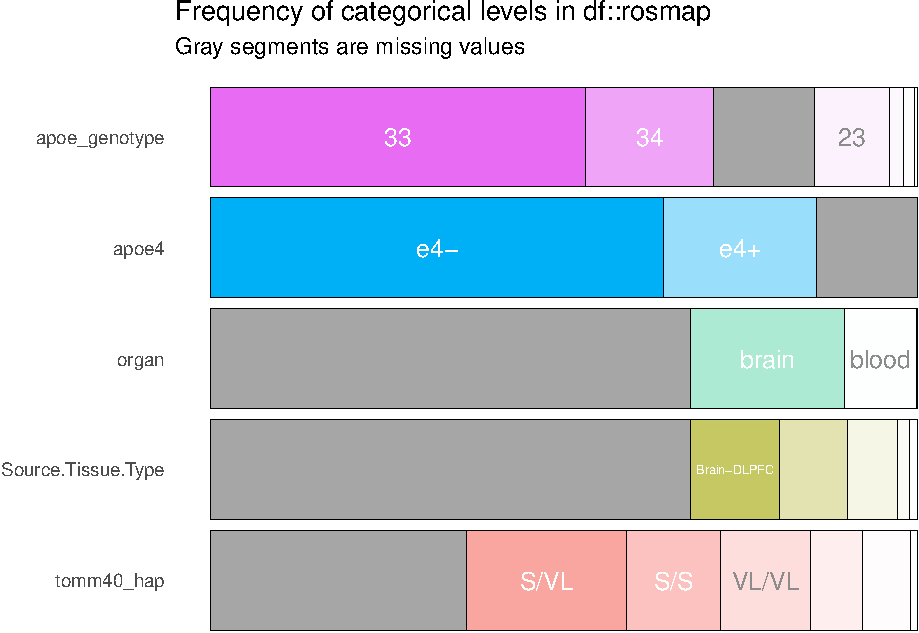
\includegraphics{notebook_files/figure-latex/unnamed-chunk-2-1.pdf}

\begin{Shaded}
\begin{Highlighting}[]
\NormalTok{demo_c }\OperatorTok\StringTok{ }\KeywordTok{show_plot}\NormalTok{(}\DataTypeTok{high_cardinality =} \DecValTok{5}\NormalTok{)}
\end{Highlighting}
\end{Shaded}

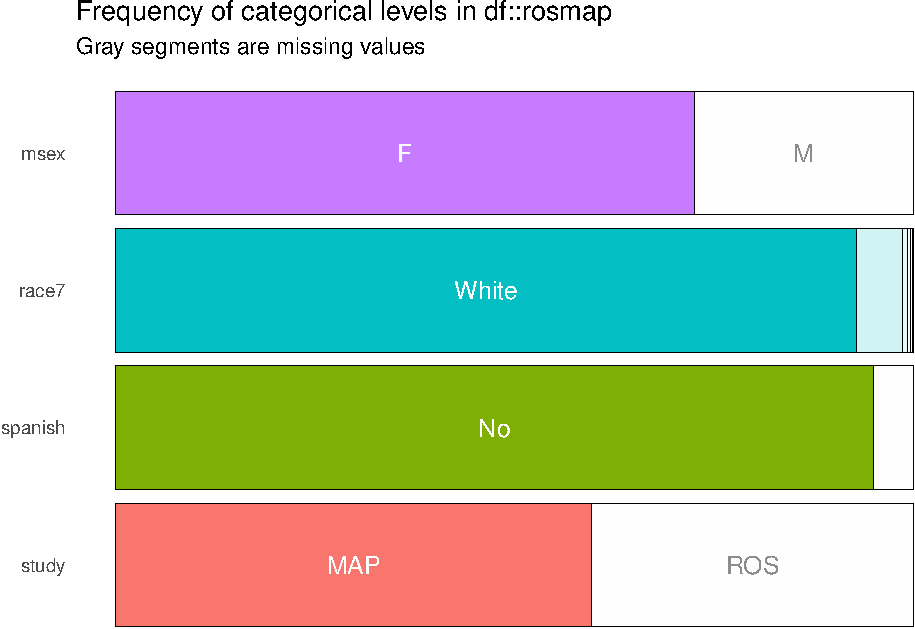
\includegraphics{notebook_files/figure-latex/unnamed-chunk-2-2.pdf}

\hypertarget{genetics}{%
\section{Genetics}\label{genetics}}

\label{tab:rosmap-genetic-global}Data Summary

variables

definitions

types

missing\_percent

unique\_count

Source.Tissue.Type

Source tissue for DNA

character

0.00

14

organ

collapsed source tissue into organ

factor

0.00

3

apoe\_genotype

APOE genotypes

factor

0.76

7

apoe4

APOE e4 carriers

factor

0.76

3

\label{tab:rosmap-genetic-factor}Variable type: Factor

col\_name

level

prop

cnt

apoe\_genotype

33

0.61

714

apoe\_genotype

34

0.22

264

apoe\_genotype

23

0.12

145

apoe\_genotype

24

0.02

22

apoe\_genotype

44

0.02

18

apoe\_genotype

NA

0.01

9

apoe\_genotype

22

0.01

7

apoe4

e4-

0.73

866

apoe4

e4+

0.26

304

apoe4

NA

0.01

9

organ

brain

0.68

796

organ

blood

0.32

378

organ

lymphocytes

0.00

5

Source.Tissue.Type

Brain-DLPFC

0.39

460

Source.Tissue.Type

Whole Blood

0.30

355

Source.Tissue.Type

Brain-Cerebellum

0.22

256

Source.Tissue.Type

Brain-Posterior Cingulate Cortex

0.06

67

Source.Tissue.Type

Other

0.03

41

\hypertarget{plots-1}{%
\subsection{Plots}\label{plots-1}}

\begin{Shaded}
\begin{Highlighting}[]
\NormalTok{genetic_c }\OperatorTok\StringTok{ }\KeywordTok{show_plot}\NormalTok{(}\DataTypeTok{high_cardinality =} \DecValTok{5}\NormalTok{)}
\end{Highlighting}
\end{Shaded}

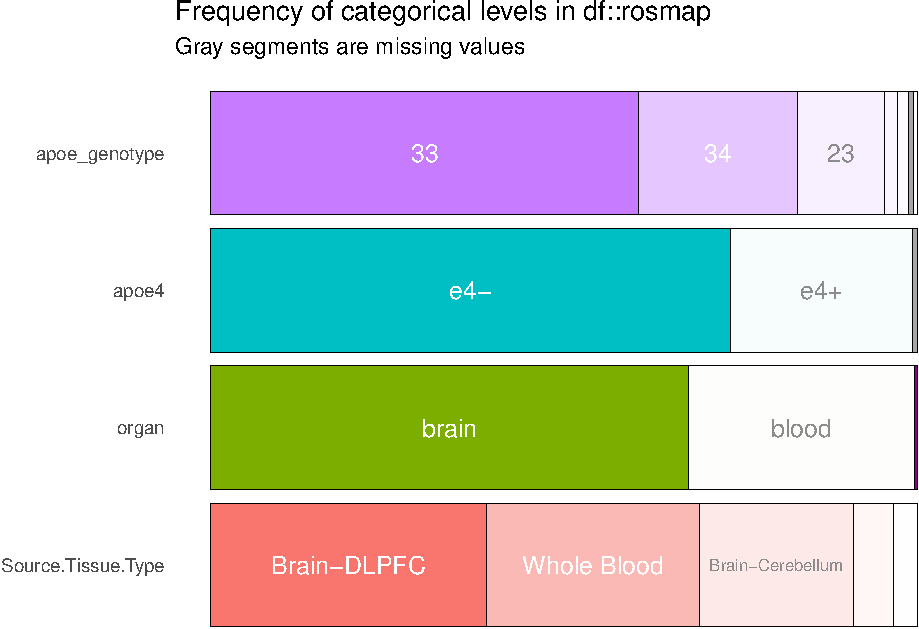
\includegraphics{notebook_files/figure-latex/unnamed-chunk-3-1.pdf}

\hypertarget{mitochondria}{%
\section{Mitochondria}\label{mitochondria}}

\label{tab:mt-numeric}Variable type: Numeric

col\_name

min

q1

median

mean

q3

max

sd

pcnt\_na

autosomal\_coverage

26.90

33.74

36.41

36.60

39.19

60.26

4.46

1.36

mt\_coverage

580.79

10103.45

25751.14

31506.63

53300.38

88911.89

23908.87

1.36

mtcn\_avg

41.37

551.39

1410.79

1733.19

2946.14

4988.99

1308.36

1.36

Quality

0.50

0.92

0.95

0.94

0.97

1.01

0.05

1.36

\label{tab:rosmap-mt-factor}Variable type: Factor

col\_name

level

prop

cnt

Haplogroup

Other

0.88

1039

Haplogroup

T2b

0.01

17

Haplogroup

H

0.01

16

Haplogroup

T1a1

0.01

16

Haplogroup

V

0.01

16

Haplogroup

NA

0.01

16

Haplogroup

H1e1a

0.01

11

Haplogroup

H1a

0.01

10

Haplogroup

H1c

0.01

10

Haplogroup

H3

0.01

10

Haplogroup

H5a1

0.01

9

Haplogroup

U5a1a1

0.01

9

macro

H

0.45

534

macro

U

0.16

186

macro

T

0.09

108

macro

J

0.09

103

macro

K

0.06

76

macro

V

0.05

54

macro

I

0.03

37

macro

X

0.02

20

macro

W

0.02

18

macro

NA

0.01

16

macro

Other

0.01

15

macro

N

0.01

12

\hypertarget{plots-2}{%
\subsection{Plots}\label{plots-2}}

\begin{Shaded}
\begin{Highlighting}[]
\NormalTok{mt_n }\OperatorTok\StringTok{ }\KeywordTok{show_plot}\NormalTok{()}
\end{Highlighting}
\end{Shaded}

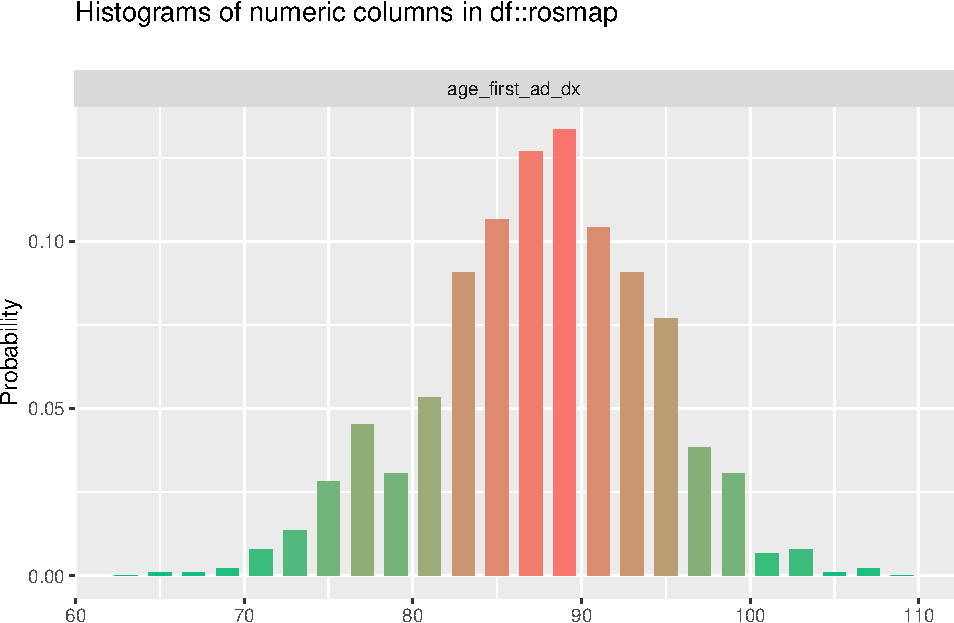
\includegraphics{notebook_files/figure-latex/unnamed-chunk-4-1.pdf}

\begin{Shaded}
\begin{Highlighting}[]
\NormalTok{mt_c }\OperatorTok\StringTok{ }\KeywordTok{show_plot}\NormalTok{(}\DataTypeTok{high_cardinality =} \DecValTok{5}\NormalTok{)}
\end{Highlighting}
\end{Shaded}

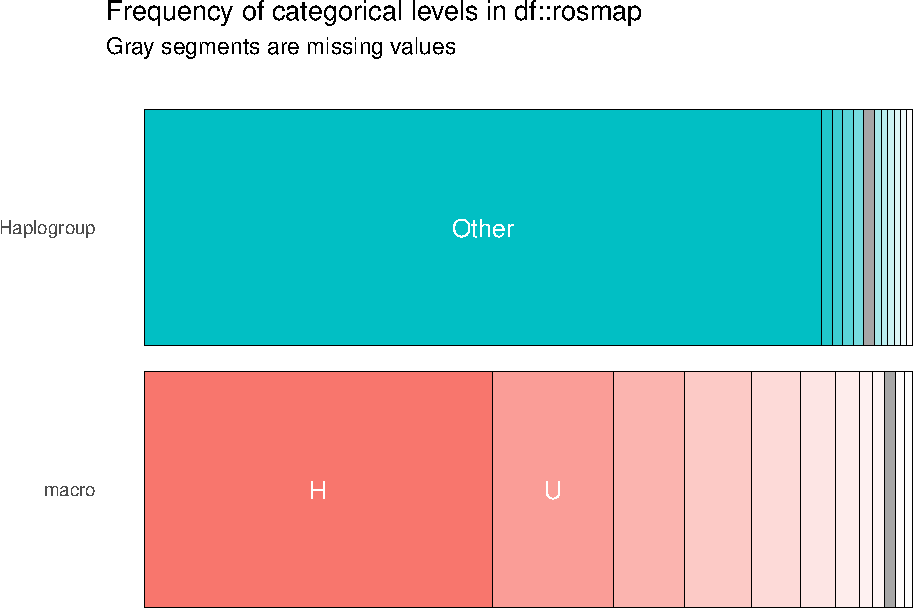
\includegraphics{notebook_files/figure-latex/unnamed-chunk-4-2.pdf}

\hypertarget{clinical-diagnosis}{%
\section{Clinical Diagnosis}\label{clinical-diagnosis}}

\begin{itemize}
\tightlist
\item
  \href{https://www.radc.rush.edu/docs/var/detail.htm?category=Clinical+Diagnosis\&subcategory=Final+consensus+diagnosis\&variable=cogdx}{Clinical cognitive diagnosis summary}: \texttt{cogdx} Physician's overall cognitive diagnostic category

  \begin{itemize}
  \tightlist
  \item
    1 = NCI: No cognitive impairment (No impaired domains)
  \item
    2 = MCI: Mild cognitive impairment (One impaired domain) and NO other cause of CI
  \item
    3 = MCI: Mild cognitive impairment (One impaired domain) AND another cause of CI
  \item
    4 = AD: Alzheimer's dementia and NO other cause of CI (NINCDS PROB AD)
  \item
    5 = AD: Alzheimer's dementia AND another cause of CI (NINCDS POSS AD)
  \item
    6 = Other dementia: Other primary cause of dementia
  \end{itemize}
\item
  \href{https://www.radc.rush.edu/docs/var/detail.htm?category=Clinical+Diagnosis\&subcategory=Dementia\&variable=age_first_ad_dx}{Age at first Alzheimer's dementia dx}: \texttt{age\_first\_ad\_dx} Age at cycle where first Alzheimer's dementia diagnosis was given
\item
  \href{https://www.radc.rush.edu/docs/var/detail.htm?category=Clinical+Diagnosis\&subcategory=Final+consensus+diagnosis\&variable=cogdx}{Final consensus cognitive diagnosis}: \texttt{dcfdx\_lv} Clinical consensus diagnosis of cognitive status at time of death - same coding as \texttt{cogdx}
\end{itemize}

\label{tab:rosmap-dx}Data Summary

variables

definitions

types

missing\_percent

unique\_count

cogdx

Physician's overall cognitive diagnostic category

factor

0.00

6

age\_first\_ad\_dx

Age at cycle where first Alzheimer's dementia diagnosis was given

numeric

65.14

392

dcfdx\_lv

Clinical consensus diagnosis of cognitive status at time of death

factor

0.00

6

\label{tab:rosmap-dx-numeric}Variable type: Numeric

col\_name

min

q1

median

mean

q3

max

sd

pcnt\_na

age\_first\_ad\_dx

68.93

83.21

87.38

87.32

91.36

107.23

6.39

65.14

\label{tab:rosmap-dx-factor}Variable type: Factor

col\_name

level

prop

cnt

cogdx

4

0.37

433

1

0.32

374

2

0.23

273

5

0.05

58

6

0.02

21

3

0.02

20

dcfdx\_lv

4

0.36

421

1

0.32

379

2

0.25

289

5

0.05

60

6

0.02

20

3

0.01

10

\hypertarget{plots-3}{%
\subsection{Plots}\label{plots-3}}

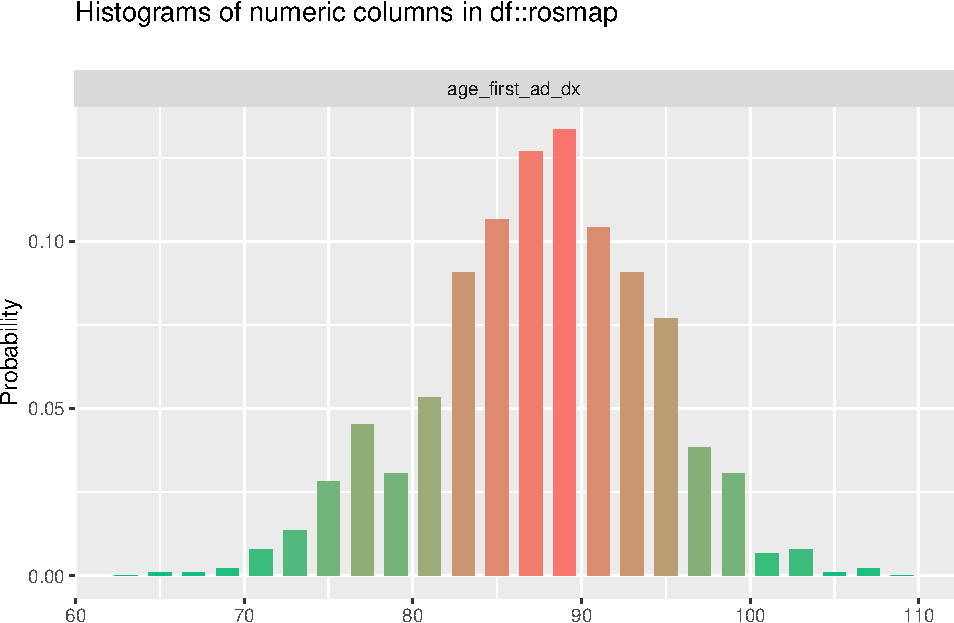
\includegraphics{notebook_files/figure-latex/unnamed-chunk-5-1.pdf} 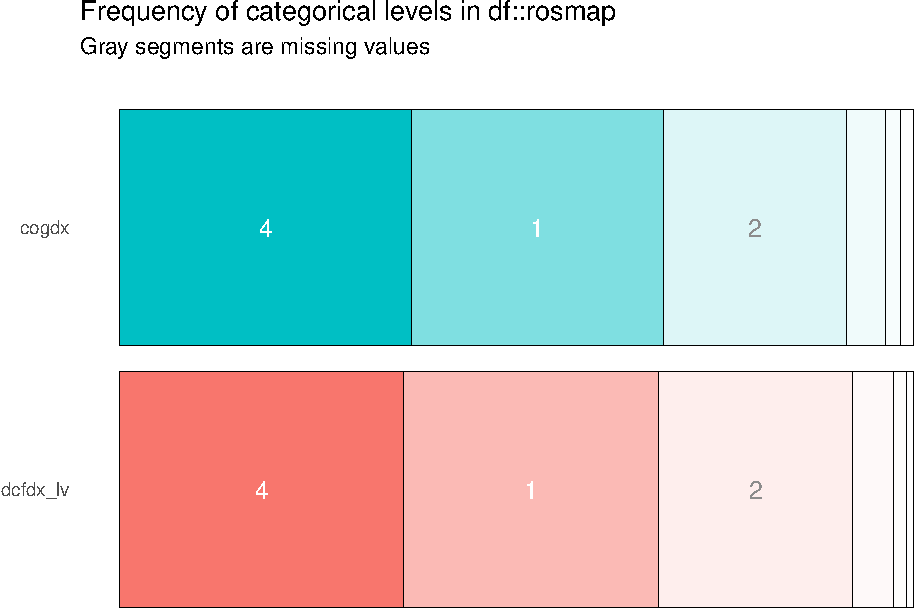
\includegraphics{notebook_files/figure-latex/unnamed-chunk-5-2.pdf}

\hypertarget{cross-tabs}{%
\subsection{Cross-tabs}\label{cross-tabs}}

\textbf{Characteristic}

1

2

3

4

5

6

\textbf{Total}

\textbf{cogdx}

1

359 (30\%)

14 (1.2\%)

0 (0\%)

1 (\textless{}0.1\%)

0 (0\%)

0 (0\%)

374 (32\%)

2

14 (1.2\%)

251 (21\%)

5 (0.4\%)

2 (0.2\%)

0 (0\%)

1 (\textless{}0.1\%)

273 (23\%)

3

4 (0.3\%)

11 (0.9\%)

4 (0.3\%)

1 (\textless{}0.1\%)

0 (0\%)

0 (0\%)

20 (1.7\%)

4

1 (\textless{}0.1\%)

13 (1.1\%)

0 (0\%)

391 (33\%)

22 (1.9\%)

6 (0.5\%)

433 (37\%)

5

0 (0\%)

0 (0\%)

0 (0\%)

17 (1.4\%)

34 (2.9\%)

7 (0.6\%)

58 (4.9\%)

6

1 (\textless{}0.1\%)

0 (0\%)

1 (\textless{}0.1\%)

9 (0.8\%)

4 (0.3\%)

6 (0.5\%)

21 (1.8\%)

\textbf{Total}

379 (32\%)

289 (25\%)

10 (0.8\%)

421 (36\%)

60 (5.1\%)

20 (1.7\%)

1179 (100\%)

\hypertarget{pathology}{%
\section{Pathology}\label{pathology}}

\href{https://www.radc.rush.edu/docs/var/overview.htm?category=Pathology}{Pathology}: post-mortem neuropathologic evaluation

\begin{itemize}
\tightlist
\item
  Alzheimer's disease

  \begin{itemize}
  \tightlist
  \item
    \href{https://www.radc.rush.edu/docs/var/detail.htm?category=Pathology\&subcategory=Alzheimer\%27s+disease\&variable=niareagansc}{NIA-Reagan diagnosis of AD}: \texttt{niareagansc} modified NIA-Reagan diagnosis of Alzheimer's disease is based on consensus recommendations for postmortem diagnosis of Alzheimer's disease. The criteria rely on both neurofibrillary tangles (Braak) and neuritic plaques (CERAD).

    \begin{itemize}
    \tightlist
    \item
      1 = High; 2 = Intermediate; 3 = Low; 4 = No AD
    \end{itemize}
  \item
    Dichomtomized NIA-Reagan: \texttt{ad\_reagan}
  \item
    \href{https://www.radc.rush.edu/docs/var/detail.htm?category=Pathology\&subcategory=Alzheimer\%27s+disease\&variable=ceradsc}{CERAD score}: \texttt{ceradsc} CERAD score is a semiquantitative measure of neuritic plaques. A CERAD neuropathologic diagnosis of AD required moderate (probable AD) or frequent neuritic plaques (definite AD) in one or more neocortical regions.

    \begin{itemize}
    \tightlist
    \item
      1 = Definite -\textgreater{} frequent (C3); 2 = Probable -\textgreater{} moderate (C2); 3 = Possible -\textgreater{} Sparse (C1); 4 = No AD -\textgreater{} None (C0)
    \end{itemize}
  \item
    \href{https://www.radc.rush.edu/docs/var/detail.htm?category=Pathology\&subcategory=Alzheimer\%27s+disease\&variable=braaksc}{Braak stage}: \texttt{braaksc} Braak Stage is a semiquantitative measure of severity of neurofibrillary tangle (NFT) pathology.

    \begin{itemize}
    \tightlist
    \item
      0 = 0; 1 = I (entorhinal); 2 = II (entorhinal); 3 = III (limbic); 4 = IV (limbic); 5 = V (neocortical); 6 = VI (neocortical)
    \end{itemize}
  \item
    \href{https://www.radc.rush.edu/docs/var/detail.htm?category=Pathology\&subcategory=Alzheimer\%27s+disease\&variable=gpath}{Global AD pathology burden}: \texttt{gpath} Global AD pathology burden is a quantitative summary of AD pathology derived from counts of three AD pathologies: neuritic plaques (n), diffuse plaques (d), and neurofibrillary tangles (nft)
  \end{itemize}
\item
  Beta-Amyloid

  \begin{itemize}
  \tightlist
  \item
    \href{https://www.radc.rush.edu/docs/var/detail.htm?category=Pathology\&subcategory=Beta-Amyloid\&variable=amyloid}{amyloid}: \texttt{amyloid} Overall amyloid level - Mean of 8 brain regions
  \item
    \href{https://www.radc.rush.edu/docs/var/detail.htm?category=Pathology\&subcategory=Beta-Amyloid\&variable=plaq_d}{plaq\_d}: \texttt{plaq\_d} Diffuse plaque summary based on 5 regions
  \item
    \href{https://www.radc.rush.edu/docs/var/detail.htm?category=Pathology\&subcategory=Beta-Amyloid\&variable=plaq_n}{plaq\_n}: \texttt{plaq\_n} Neuritic plaque summary based on 5 regions
  \end{itemize}
\item
  PHF tau Tangles

  \begin{itemize}
  \tightlist
  \item
    \href{https://www.radc.rush.edu/docs/var/detail.htm?category=Pathology\&subcategory=PHF+tau+tangles\&variable=tangles}{Tangle}: \texttt{tangles} Tangle density - Mean of 8 brain regions
  \item
    \href{https://www.radc.rush.edu/docs/var/detail.htm?category=Pathology\&subcategory=PHF+tau+tangles\&variable=nft}{NFT burden}: \texttt{nft} Neurofibrillary tangle summary based on 5 regions
  \end{itemize}
\item
  \href{https://www.radc.rush.edu/docs/var/detail.htm?category=Pathology\&subcategory=Lewy+body\%2fPD\&variable=dlbdx}{Lewy Body disease}: \texttt{dlbdx} Pathologic diagnosis of Lewy body diseases - 4 stages

  \begin{itemize}
  \tightlist
  \item
    0 = Not present; 1 = nigral-predominant; 2 = limbic-type; 3 = neocortical-type
  \end{itemize}
\item
  Vascular

  \begin{itemize}
  \tightlist
  \item
    \href{https://www.radc.rush.edu/docs/var/detail.htm?category=Pathology\&subcategory=Vascular+-+Infarcts+(Presence+of)\&variable=ci_num2_gct}{gross infarcts}: \texttt{ci\_num\_gct} Cerebral Infarctions - Binary - Gross-Chronic-Any Location
  \item
    \href{https://www.radc.rush.edu/docs/var/detail.htm?category=Pathology\&subcategory=Vascular+-+Infarcts+(Presence+of)\&variable=ci_num2_mct}{micro infarcts}: \texttt{ci\_num2\_mct} Cerebral Infarctions - Binary - Micro-Chronic-Any Location
  \item
    \href{https://www.radc.rush.edu/docs/var/detail.htm?category=Pathology\&subcategory=Vascular+-+General+measures\&variable=cvda_4gp2}{Cerebral atherosclerosis}: \texttt{cvda\_4gp2} Cerebral Atherosclerosis Rating

    \begin{itemize}
    \tightlist
    \item
      0 = None; 1 = Mild; 2 = Moderate; 3 = Severe
    \end{itemize}
  \item
    \href{https://www.radc.rush.edu/docs/var/detail.htm?category=Pathology\&subcategory=Vascular+-+General+measures\&variable=caa_4gp}{Cerebral amyloid angiopathy}: \texttt{caa\_4gp} Cerebral amyloid angiopathy

    \begin{itemize}
    \tightlist
    \item
      0 = None; 1 = Mild; 2 = Moderate; 3 = Severe
    \end{itemize}
  \item
    \href{https://www.radc.rush.edu/docs/var/detail.htm?category=Pathology\&subcategory=Vascular+-+General+measures\&variable=arteriol_scler}{Arteriolosclerosis}: \texttt{arteriol\_scler} Arteriolosclerosis

    \begin{itemize}
    \tightlist
    \item
      0 = None; 1 = Mild; 2 = Moderate; 3 = Severe
    \end{itemize}
  \end{itemize}
\item
  \href{https://www.radc.rush.edu/docs/var/detail.htm?category=Pathology\&subcategory=Hippocampal+sclerosis\&variable=hspath_typ}{Hippocampal sclerosis (Typical)}: \texttt{hspath\_typ} Definite presence of typical hippocampal sclerosis
\item
  \href{https://www.radc.rush.edu/docs/var/detail.htm?category=Pathology\&subcategory=TDP-43\&variable=tdp_st4}{TDP-43 stage}: \texttt{tdp\_st4} TDP-43 pathology from 8 regions

  \begin{itemize}
  \tightlist
  \item
    0 = None; 1 = Amygdala; 2 = Amygdala + Limbic; 3 = Amygdala + Limbic + Neocortical
  \end{itemize}
\end{itemize}

\label{tab:rosmap-path}Data Summary

variables

definitions

types

missing\_percent

unique\_count

niareagansc

NA

ordered

0.00

4

ceradsc

NA

ordered

0.00

4

braaksc

NA

ordered

0.00

7

gpath

NA

numeric

0.00

1121

amyloid

NA

numeric

0.68

990

plaq\_d

NA

numeric

0.00

910

plaq\_n

NA

numeric

0.00

879

tangles

NA

numeric

1.02

1151

nft

NA

numeric

0.00

979

dlbdx

NA

factor

3.31

5

ci\_num2\_gct

NA

factor

0.00

2

ci\_num2\_mct

NA

factor

0.00

2

cvda\_4gp2

NA

factor

0.59

5

caa\_4gp

NA

factor

3.05

5

arteriol\_scler

NA

factor

0.68

5

hspath\_typ

NA

factor

0.85

3

tdp\_st4

NA

factor

8.40

5

\label{tab:rosmap-path-numeric}Variable type: Numeric

col\_name

min

q1

median

mean

q3

max

sd

pcnt\_na

gpath

0

0.19

0.66

0.76

1.17

2.95

0.63

0.00

amyloid

0

0.62

3.05

4.26

6.67

22.94

4.23

0.68

plaq\_d

0

0.08

0.58

0.79

1.18

4.91

0.82

0.00

plaq\_n

0

0.06

0.71

0.84

1.33

5.01

0.83

0.00

tangles

0

1.49

4.01

6.65

8.56

61.01

7.76

1.02

nft

0

0.13

0.37

0.65

0.86

6.16

0.76

0.00

\hypertarget{htmlwidget-21b10f0fd53e619dc699}{}

\hypertarget{plots-4}{%
\subsection{Plots}\label{plots-4}}

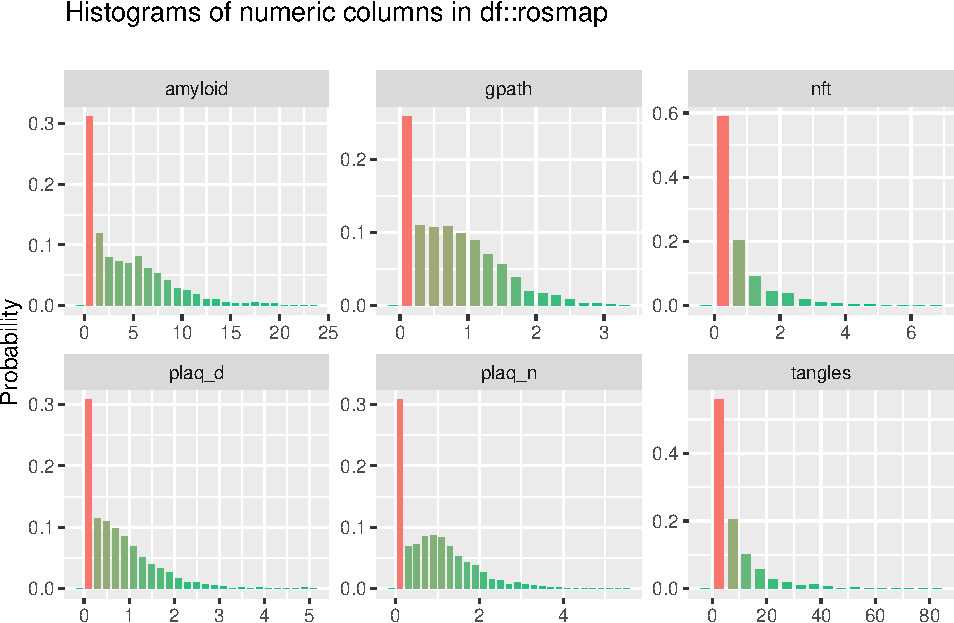
\includegraphics{notebook_files/figure-latex/rosmap-inspect-plot-1.pdf} 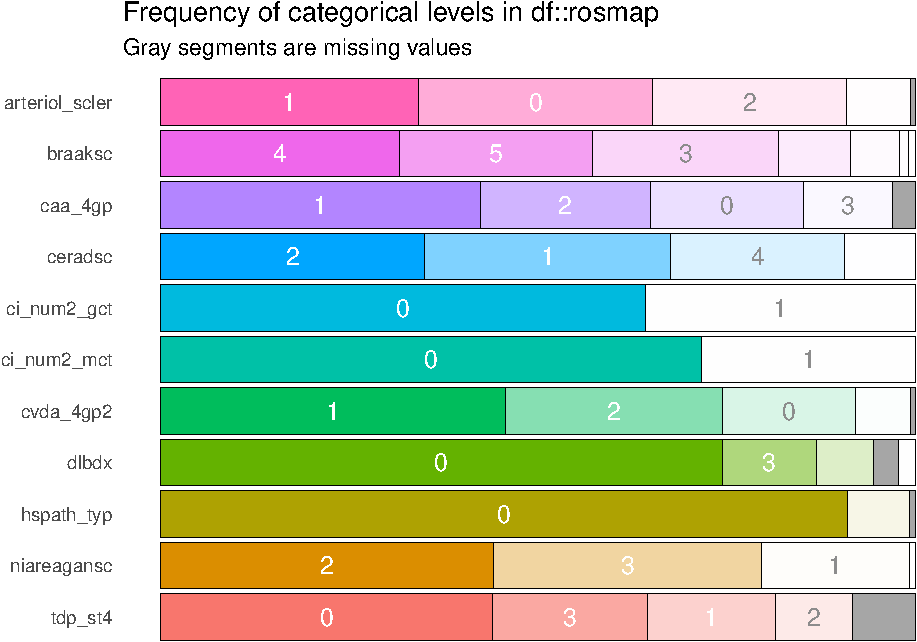
\includegraphics{notebook_files/figure-latex/rosmap-inspect-plot-2.pdf}

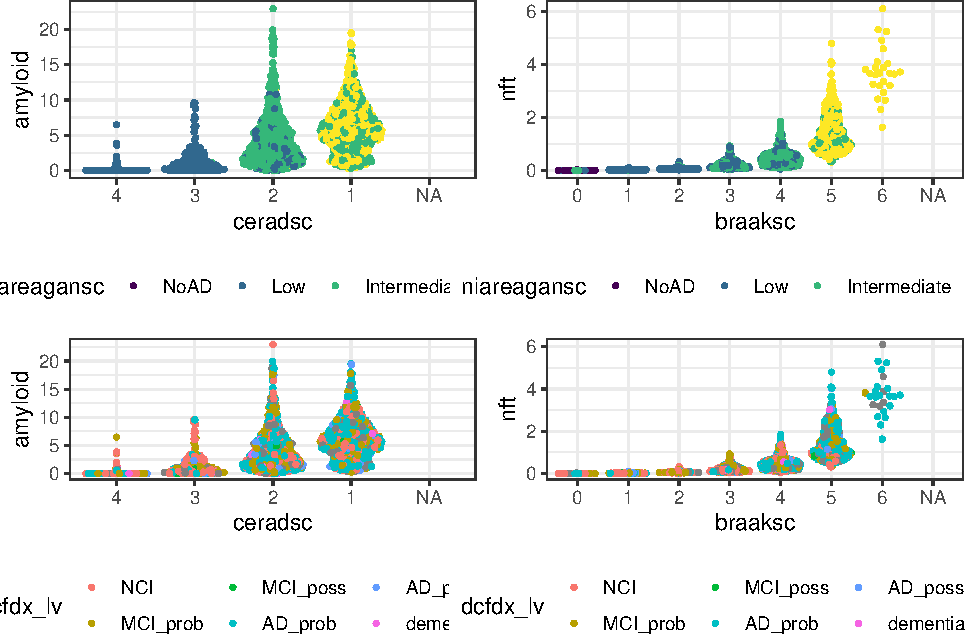
\includegraphics{notebook_files/figure-latex/rosmap-path-dx-plot-1.pdf}

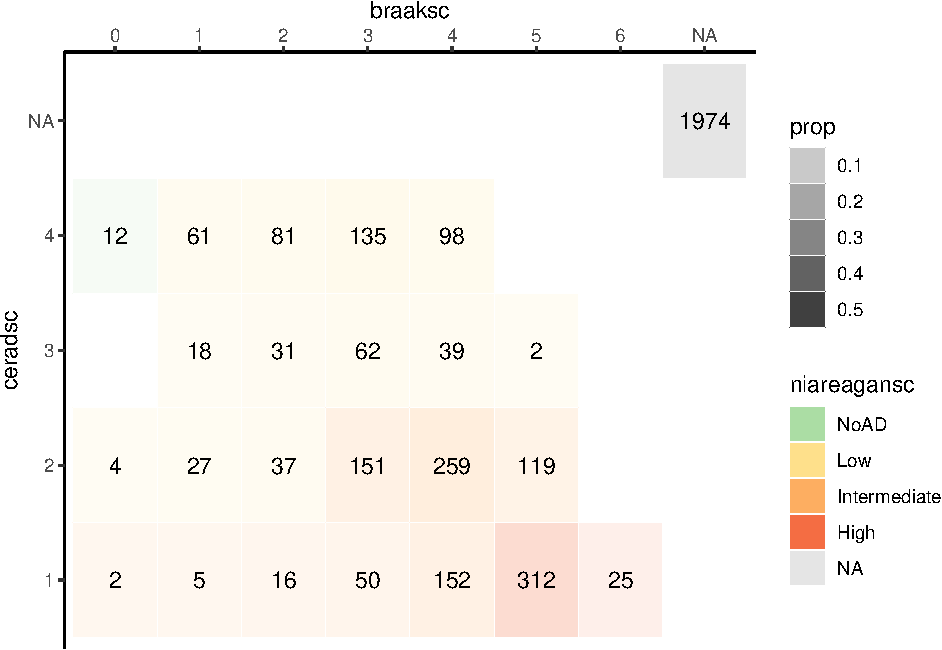
\includegraphics{notebook_files/figure-latex/rosmap-path-crosstab-plot-1.pdf}

\hypertarget{cross-tabs-1}{%
\subsection{Cross-Tabs}\label{cross-tabs-1}}

\textbf{Characteristic}

0

1

2

3

4

5

6

\textbf{Total}

\textbf{ceradsc}

4

10 (0.8\%)

42 (3.6\%)

52 (4.4\%)

104 (8.8\%)

64 (5.4\%)

0 (0\%)

0 (0\%)

272 (23\%)

3

0 (0\%)

12 (1.0\%)

23 (2.0\%)

47 (4.0\%)

27 (2.3\%)

1 (\textless{}0.1\%)

0 (0\%)

110 (9.3\%)

2

3 (0.3\%)

19 (1.6\%)

26 (2.2\%)

105 (8.9\%)

174 (15\%)

86 (7.3\%)

0 (0\%)

413 (35\%)

1

1 (\textless{}0.1\%)

3 (0.3\%)

12 (1.0\%)

34 (2.9\%)

109 (9.2\%)

214 (18\%)

11 (0.9\%)

384 (33\%)

\textbf{Total}

14 (1.2\%)

76 (6.4\%)

113 (9.6\%)

290 (25\%)

374 (32\%)

301 (26\%)

11 (0.9\%)

1179 (100\%)

\textbf{Characteristic}

4

3

2

1

\textbf{Total}

\textbf{cogdx}

1

6 (1.6\%)

208 (56\%)

144 (39\%)

16 (4.3\%)

374 (100\%)

2

4 (1.5\%)

105 (38\%)

133 (49\%)

31 (11\%)

273 (100\%)

3

0 (0\%)

11 (55\%)

7 (35\%)

2 (10\%)

20 (100\%)

4

0 (0\%)

60 (14\%)

206 (48\%)

167 (39\%)

433 (100\%)

5

0 (0\%)

25 (43\%)

22 (38\%)

11 (19\%)

58 (100\%)

6

0 (0\%)

10 (48\%)

8 (38\%)

3 (14\%)

21 (100\%)

\textbf{Total}

10 (0.8\%)

419 (36\%)

520 (44\%)

230 (20\%)

1179 (100\%)

ceradsc

braaksc

NoAD

Low

Intermediate

High

C0

B0

10

NA

NA

NA

B1

NA

94

NA

NA

B2

NA

168

NA

NA

C1

B1

NA

35

NA

NA

B2

NA

73

1

NA

B3

NA

1

NA

NA

C2

B0

NA

3

NA

NA

B1

NA

44

1

NA

B2

NA

1

278

NA

B3

NA

NA

82

4

C3

B0

NA

NA

1

NA

B1

NA

NA

15

NA

B2

NA

NA

142

1

B3

NA

NA

NA

225

\hypertarget{cognition}{%
\section{Cognition}\label{cognition}}

\href{https://www.radc.rush.edu/docs/var/detail.htm?category=Cognition\&subcategory=Test+scores\&variable=cts_mmse30}{mmse}: Mini Mental State Examination is a widely used, 30 item, standardized screening measure of dementia severity. The MMSE can be used as a surrogate measure for the CDR for the staging of dementia in AD \href{https://doi.org/10.1097/01.JGP.0000192478.82189.a8}{Perneczky et al 2006}.

\begin{longtable}[]{@{}ll@{}}
\toprule
MMSE & CDR\tabularnewline
\midrule
\endhead
30 & 0 (No)\tabularnewline
26-29 & 0.5 (Questionable)\tabularnewline
21-25 & 1 (Mild)\tabularnewline
11-20 & 2 (Moderate)\tabularnewline
0-10 & 3 (Severe)\tabularnewline
\bottomrule
\end{longtable}

\begin{verbatim}
# A tibble: 2 x 6
  variables     types   missing_count missing_percent unique_count unique_rate
  <chr>         <chr>           <int>           <dbl>        <int>       <dbl>
1 cts_mmse30_lv numeric             2           0.170           84     0.0712 
2 CDR           factor              2           0.170            6     0.00509
\end{verbatim}

\label{tab:rosmap-cog-numeric}Variable type: Numeric

col\_name

min

q1

median

mean

q3

max

sd

pcnt\_na

cts\_mmse30\_lv

0

15.56

25

20.84

28

30

9.2

0.17

\hypertarget{htmlwidget-b4007d8949fefc4d49ed}{}

\hypertarget{plots-5}{%
\subsection{Plots}\label{plots-5}}

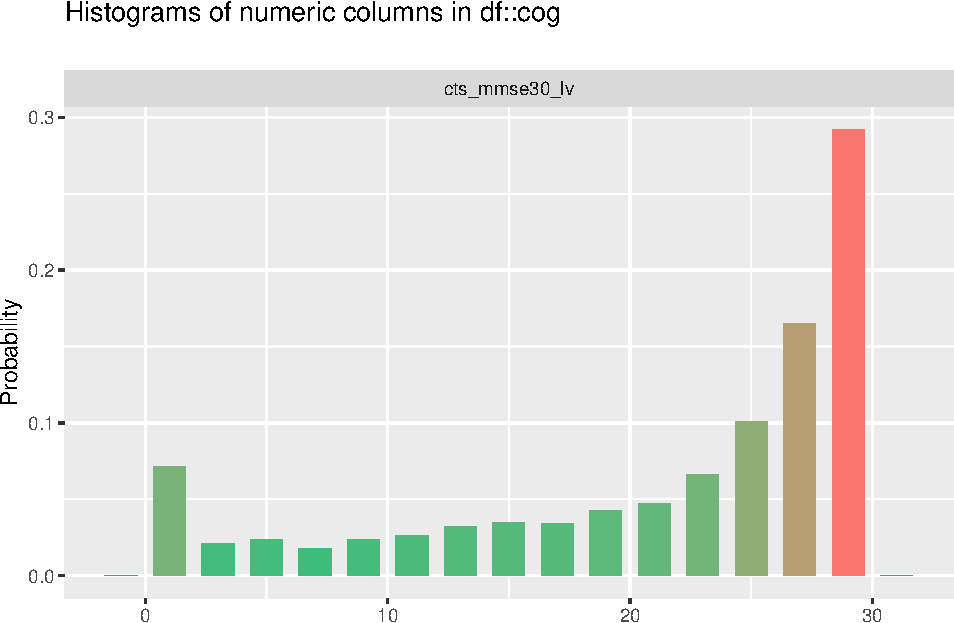
\includegraphics{notebook_files/figure-latex/unnamed-chunk-10-1.pdf} 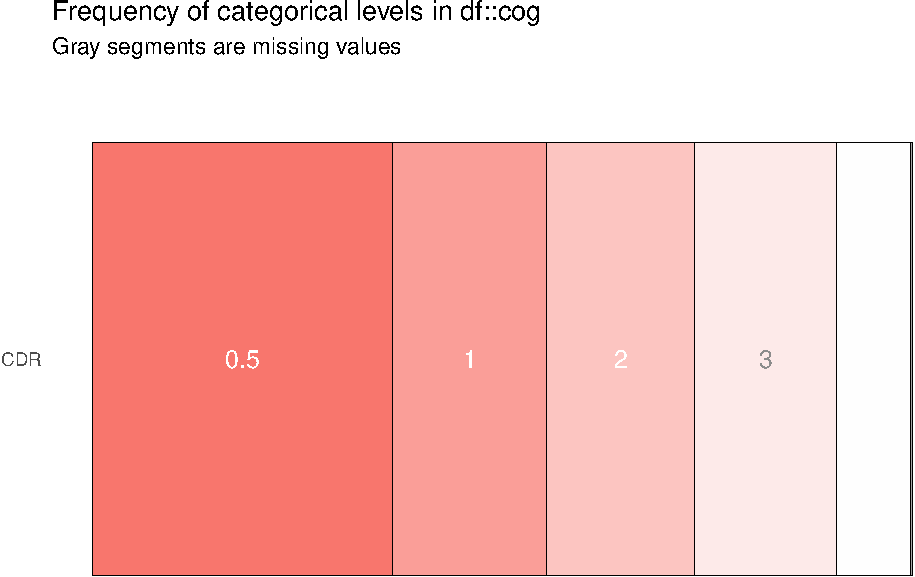
\includegraphics{notebook_files/figure-latex/unnamed-chunk-10-2.pdf}

\hypertarget{msbb}{%
\chapter{MSBB}\label{msbb}}

Samples come from 364 postmortem control, mild cognitive impaired (MCI) and AD brains with rich clinical and pathophysiological data from the Mount Sinai/JJ Peters VA Medical Center Brain Bank (MSBB--Mount Sinai NIH Neurobiobank) cohort. The majority (301) of the samples were of European ancestry, while 36 were African American, 25 were Latino, one was Asian, and one was unknown for race. Neuropathological assessments were performed using CERAD scores and Braak Staging. The CDR scale was conducted for assessment of dementia and cognitive status (\citet{10.1038/sdata.2018.185}).

Clinical Code Book: \href{https://adknowledgeportal.synapse.org/Explore/Studies?Study=syn3159438}{Synapse}

\begin{Shaded}
\begin{Highlighting}[]
\CommentTok{## MSBB}
\NormalTok{msbb.raw1 <-}\StringTok{ }\KeywordTok{read_tsv}\NormalTok{(}\StringTok{'data/AMPAD/msbb/WGS_Metadata.txt'}\NormalTok{) }
\NormalTok{msbb.raw2 <-}\StringTok{ }\KeywordTok{read_tsv}\NormalTok{(}\StringTok{'data/AMPAD_extra/msbb.wgs.meta.tsv'}\NormalTok{)}
\NormalTok{msbb.path <-}\StringTok{ }\NormalTok{readxl}\OperatorTok{::}\KeywordTok{read_xlsx}\NormalTok{(}\StringTok{'data/AMPAD_extra/msbb/TempAmp_AD-Shea-2-2020.xlsx'}\NormalTok{, }\DataTypeTok{sheet =} \DecValTok{2}\NormalTok{) }\OperatorTok\StringTok{ }
\StringTok{  }\KeywordTok{mutate}\NormalTok{(}\DataTypeTok{id =} \KeywordTok{as.character}\NormalTok{(id))}
\NormalTok{msbb.raw <-}\StringTok{ }\NormalTok{msbb.raw1 }\OperatorTok\StringTok{ }
\StringTok{  }\KeywordTok{select}\NormalTok{(WGS, individualIdentifier, PMI, RACE, CDR, SEX, NP}\FloatTok{.1}\NormalTok{, PlaqueMean, bbscore) }\OperatorTok
\StringTok{  }\KeywordTok{left_join}\NormalTok{(}\KeywordTok{select}\NormalTok{(msbb.raw2, Libid, AOD, APOE_inferred), }\DataTypeTok{by =} \KeywordTok{c}\NormalTok{(}\StringTok{'WGS'}\NormalTok{ =}\StringTok{ 'Libid'}\NormalTok{)) }\OperatorTok\StringTok{ }
\StringTok{  }\KeywordTok{mutate}\NormalTok{(}\DataTypeTok{SubNum =} \KeywordTok{str_extract}\NormalTok{(}\KeywordTok{gsub}\NormalTok{(}\StringTok{"(?<![0-9])0+"}\NormalTok{, }\StringTok{""}\NormalTok{, individualIdentifier, }\DataTypeTok{perl =} \OtherTok{TRUE}\NormalTok{), }\StringTok{'[:digit:].*'}\NormalTok{)) }\OperatorTok\StringTok{ }
\StringTok{  }\KeywordTok{left_join}\NormalTok{(msbb.path, }\DataTypeTok{by =} \KeywordTok{c}\NormalTok{(}\StringTok{'SubNum'}\NormalTok{ =}\StringTok{ 'id'}\NormalTok{)) }\OperatorTok
\StringTok{  }\KeywordTok{mutate}\NormalTok{(}\DataTypeTok{study =} \StringTok{'MSBB'}\NormalTok{, }
         \DataTypeTok{WGS =} \KeywordTok{as.character}\NormalTok{(WGS))}

\NormalTok{mosdepth <-}\StringTok{ }\KeywordTok{read_tsv}\NormalTok{(}\StringTok{'data/mosdepth/mosdepth_all.txt'}\NormalTok{)}
\NormalTok{haplogrep <-}\StringTok{ }\KeywordTok{read_tsv}\NormalTok{(}\StringTok{'data/haplogrep/haplogrep_all.txt'}\NormalTok{)}
\end{Highlighting}
\end{Shaded}

\begin{Shaded}
\begin{Highlighting}[]
\CommentTok{## Recode NP.1 -> ceradsc to be consistent with ROSMAP}
\NormalTok{msbb <-}\StringTok{ }\NormalTok{msbb.raw }\OperatorTok
\StringTok{  }\KeywordTok{left_join}\NormalTok{(haplogrep, }\DataTypeTok{by =} \KeywordTok{c}\NormalTok{(}\StringTok{'WGS'}\NormalTok{ =}\StringTok{ 'SampleID'}\NormalTok{)) }\OperatorTok
\StringTok{  }\KeywordTok{left_join}\NormalTok{(mosdepth, }\DataTypeTok{by =} \KeywordTok{c}\NormalTok{(}\StringTok{'WGS'}\NormalTok{ =}\StringTok{ 'SampleID'}\NormalTok{)) }\OperatorTok
\StringTok{  }\KeywordTok{mutate}\NormalTok{(}\DataTypeTok{id =} \KeywordTok{paste0}\NormalTok{(}\StringTok{'MSBB'}\NormalTok{, WGS)) }\OperatorTok
\StringTok{  }\KeywordTok{mutate}\NormalTok{(}\DataTypeTok{APOE_inferred =} \KeywordTok{recode}\NormalTok{(APOE_inferred, }\StringTok{'e2/e2'}\NormalTok{ =}\StringTok{ '22'}\NormalTok{, }\StringTok{'e2/e3'}\NormalTok{ =}\StringTok{ '23'}\NormalTok{, }\StringTok{'e3/e3'}\NormalTok{ =}\StringTok{ '33'}\NormalTok{, }\StringTok{'e2/e4'}\NormalTok{ =}\StringTok{ '24'}\NormalTok{, }\StringTok{'e3/e4'}\NormalTok{ =}\StringTok{ '34'}\NormalTok{, }\StringTok{'e4/e4'}\NormalTok{ =}\StringTok{ '44'}\NormalTok{),}
        \DataTypeTok{apoe4 =} \KeywordTok{recode}\NormalTok{(APOE_inferred, }\StringTok{'22'}\NormalTok{ =}\StringTok{ 'e4-'}\NormalTok{, }\StringTok{'23'}\NormalTok{ =}\StringTok{ 'e4-'}\NormalTok{, }\StringTok{'33'}\NormalTok{ =}\StringTok{ 'e4-'}\NormalTok{, }\StringTok{'24'}\NormalTok{ =}\StringTok{ 'e4+'}\NormalTok{, }\StringTok{'34'}\NormalTok{ =}\StringTok{ 'e4+'}\NormalTok{, }\StringTok{'44'}\NormalTok{ =}\StringTok{ 'e4+'}\NormalTok{),}
        \DataTypeTok{SEX =} \KeywordTok{as.factor}\NormalTok{(SEX), }
        \DataTypeTok{SourceTissue =} \StringTok{'prefrontal cortex'}\NormalTok{,}
        \DataTypeTok{APOE_inferred =} \KeywordTok{as.factor}\NormalTok{(APOE_inferred), }
        \DataTypeTok{apoe4 =} \KeywordTok{as.factor}\NormalTok{(apoe4), }
        \DataTypeTok{RACE =} \KeywordTok{as.factor}\NormalTok{(RACE), }
        \DataTypeTok{z_mtdnacn =} \KeywordTok{scale}\NormalTok{(mtcn_avg, }\DataTypeTok{center =} \OtherTok{TRUE}\NormalTok{, }\DataTypeTok{scale =} \OtherTok{TRUE}\NormalTok{)[,}\DecValTok{1}\NormalTok{],}
        \DataTypeTok{cerad =} \KeywordTok{recode}\NormalTok{(NP}\FloatTok{.1}\NormalTok{, }\StringTok{'1'}\NormalTok{ =}\StringTok{ 'Normal'}\NormalTok{, }\StringTok{'2'}\NormalTok{ =}\StringTok{ 'Definite'}\NormalTok{, }\StringTok{'3'}\NormalTok{ =}\StringTok{ 'Probable'}\NormalTok{, }\StringTok{'4'}\NormalTok{ =}\StringTok{ 'Possible'}\NormalTok{),}
        \DataTypeTok{cerad =} \KeywordTok{ordered}\NormalTok{(cerad, }\DataTypeTok{levels =} \KeywordTok{c}\NormalTok{(}\StringTok{'Normal'}\NormalTok{, }\StringTok{'Possible'}\NormalTok{, }\StringTok{'Probable'}\NormalTok{, }\StringTok{'Definite'}\NormalTok{)),}
        \DataTypeTok{ceradsc =} \KeywordTok{pmax}\NormalTok{(HippoPlaquesWCoresValue, EntorPlaquesWCoresValue, MidPlaquesWCoresValue, }
\NormalTok{                       SupPlaquesWCoresValue, InfPlaquesWCoresValue, OcciPlaquesWCoresValue),}
        \DataTypeTok{ceradsc =} \KeywordTok{ordered}\NormalTok{(ceradsc),}
        \DataTypeTok{ceradsc =} \KeywordTok{fct_recode}\NormalTok{(ceradsc, }\StringTok{'4'}\NormalTok{ =}\StringTok{ '0'}\NormalTok{, }\StringTok{'3'}\NormalTok{ =}\StringTok{ '1'}\NormalTok{, }\StringTok{'2'}\NormalTok{ =}\StringTok{ '3'}\NormalTok{, }\StringTok{'1'}\NormalTok{ =}\StringTok{ '5'}\NormalTok{),}
        \DataTypeTok{bbscore =} \KeywordTok{ordered}\NormalTok{(bbscore, }\DataTypeTok{levels =} \KeywordTok{c}\NormalTok{(}\StringTok{'0'}\NormalTok{, }\StringTok{'1'}\NormalTok{, }\StringTok{'2'}\NormalTok{, }\StringTok{'3'}\NormalTok{, }\StringTok{'4'}\NormalTok{, }\StringTok{'5'}\NormalTok{, }\StringTok{'6'}\NormalTok{)),}
        \DataTypeTok{niareagansc =} \KeywordTok{case_when}\NormalTok{(}
\NormalTok{          ceradsc }\OperatorTok{==}\StringTok{ }\DecValTok{4} \OperatorTok{&}\StringTok{ }\NormalTok{bbscore }\OperatorTok{==}\StringTok{ }\DecValTok{0} \OperatorTok{~}\StringTok{ }\DecValTok{4}\NormalTok{, }
\NormalTok{          ceradsc }\OperatorTok{==}\StringTok{ }\DecValTok{4} \OperatorTok{&}\StringTok{ }\NormalTok{bbscore }\OperatorTok\StringTok{ }\KeywordTok{c}\NormalTok{(}\DecValTok{1}\OperatorTok{:}\DecValTok{6}\NormalTok{) }\OperatorTok{~}\StringTok{ }\DecValTok{3}\NormalTok{, }
\NormalTok{          ceradsc }\OperatorTok{==}\StringTok{ }\DecValTok{3} \OperatorTok{&}\StringTok{ }\NormalTok{bbscore }\OperatorTok\StringTok{ }\KeywordTok{c}\NormalTok{(}\DecValTok{0}\OperatorTok{:}\DecValTok{6}\NormalTok{) }\OperatorTok{~}\StringTok{ }\DecValTok{3}\NormalTok{, }
\NormalTok{          ceradsc }\OperatorTok{==}\StringTok{ }\DecValTok{2} \OperatorTok{&}\StringTok{ }\NormalTok{bbscore }\OperatorTok\StringTok{ }\KeywordTok{c}\NormalTok{(}\DecValTok{0}\OperatorTok{:}\DecValTok{2}\NormalTok{) }\OperatorTok{~}\StringTok{ }\DecValTok{3}\NormalTok{,}
\NormalTok{          ceradsc }\OperatorTok{==}\StringTok{ }\DecValTok{2} \OperatorTok{&}\StringTok{ }\NormalTok{bbscore }\OperatorTok\StringTok{ }\KeywordTok{c}\NormalTok{(}\DecValTok{3}\OperatorTok{:}\DecValTok{6}\NormalTok{) }\OperatorTok{~}\StringTok{ }\DecValTok{2}\NormalTok{,}
\NormalTok{          ceradsc }\OperatorTok{==}\StringTok{ }\DecValTok{1} \OperatorTok{&}\StringTok{ }\NormalTok{bbscore }\OperatorTok\StringTok{ }\KeywordTok{c}\NormalTok{(}\DecValTok{0}\OperatorTok{:}\DecValTok{4}\NormalTok{) }\OperatorTok{~}\StringTok{ }\DecValTok{2}\NormalTok{,}
\NormalTok{          ceradsc }\OperatorTok{==}\StringTok{ }\DecValTok{1} \OperatorTok{&}\StringTok{ }\NormalTok{bbscore }\OperatorTok\StringTok{ }\KeywordTok{c}\NormalTok{(}\DecValTok{5}\OperatorTok{:}\DecValTok{6}\NormalTok{) }\OperatorTok{~}\StringTok{ }\DecValTok{1}\NormalTok{,}
\NormalTok{        ), }
        \DataTypeTok{niareagansc =} \KeywordTok{ordered}\NormalTok{(niareagansc, }\DataTypeTok{levels =} \KeywordTok{c}\NormalTok{(}\StringTok{'4'}\NormalTok{, }\StringTok{'3'}\NormalTok{, }\StringTok{'2'}\NormalTok{, }\StringTok{'1'}\NormalTok{)),}
        \DataTypeTok{ad_reagan =} \KeywordTok{fct_recode}\NormalTok{(niareagansc, }\StringTok{"1"}\NormalTok{ =}\StringTok{ "1"}\NormalTok{, }\StringTok{"1"}\NormalTok{ =}\StringTok{ "2"}\NormalTok{, }\StringTok{"0"}\NormalTok{ =}\StringTok{ "3"}\NormalTok{, }\StringTok{"0"}\NormalTok{ =}\StringTok{ "4"}\NormalTok{),}
        \DataTypeTok{braaksc_B =} \KeywordTok{fct_recode}\NormalTok{(bbscore, }\DataTypeTok{B0 =} \StringTok{"0"}\NormalTok{, }\DataTypeTok{B1 =} \StringTok{"1"}\NormalTok{, }\DataTypeTok{B1 =} \StringTok{"2"}\NormalTok{, }\DataTypeTok{B2 =} \StringTok{"3"}\NormalTok{, }\DataTypeTok{B2 =} \StringTok{"4"}\NormalTok{, }\DataTypeTok{B3 =} \StringTok{"5"}\NormalTok{, }\DataTypeTok{B3 =} \StringTok{"6"}\NormalTok{), }
        \DataTypeTok{ceradsc_C =} \KeywordTok{fct_recode}\NormalTok{(ceradsc, }\DataTypeTok{C0 =} \StringTok{"1"}\NormalTok{, }\DataTypeTok{C1 =} \StringTok{"2"}\NormalTok{, }\DataTypeTok{C2 =} \StringTok{"3"}\NormalTok{, }\DataTypeTok{C3 =} \StringTok{"4"}\NormalTok{)) }\OperatorTok
\StringTok{  }\KeywordTok{mutate_at}\NormalTok{(}\KeywordTok{vars}\NormalTok{(HippoPlaquesWCoresValue, EntorPlaquesWCoresValue, MidPlaquesWCoresValue, }
\NormalTok{                       SupPlaquesWCoresValue, InfPlaquesWCoresValue, OcciPlaquesWCoresValue), }
\NormalTok{            ordered) }\OperatorTok
\StringTok{  }\KeywordTok{select}\NormalTok{(id, study, }\DataTypeTok{sex =}\NormalTok{ SEX, }\DataTypeTok{race =}\NormalTok{ RACE, SourceTissue, PMI, NP}\FloatTok{.1}\NormalTok{, cerad, niareagansc, ad_reagan, ceradsc, HippoPlaquesWCoresValue, EntorPlaquesWCoresValue, MidPlaquesWCoresValue, SupPlaquesWCoresValue, InfPlaquesWCoresValue, OcciPlaquesWCoresValue, }\DataTypeTok{braaksc =}\NormalTok{ bbscore, braaksc_B, ceradsc_C, }\DataTypeTok{apoe =}\NormalTok{ APOE_inferred, apoe4, }\DataTypeTok{aod =}\NormalTok{ AOD, }\DataTypeTok{cdr =}\NormalTok{ CDR, PlaqueMean, mtcn_avg, z_mtdnacn, Haplogroup, Quality, macro)}

\KeywordTok{saveRDS}\NormalTok{(msbb, }\StringTok{'output/msbb.rds'}\NormalTok{)}
\end{Highlighting}
\end{Shaded}

\hypertarget{pathology-1}{%
\section{Pathology}\label{pathology-1}}

\textbf{Amyloid}

\begin{itemize}
\tightlist
\item
  \texttt{HippoPlaquesWCoresValue}, \texttt{EntorPlaquesWCoresValue}, \texttt{MidPlaquesWCoresValue}, \texttt{SupPlaquesWCoresValue}, \texttt{InfPlaquesWCoresValue}, \texttt{OcciPlaquesWCoresValue}: Neuritic plaque burden measured in 8 brain regions. (0 = Absent; 1 = Sparese; 3 = Moderate; 5 = Frequent)

  \begin{itemize}
  \tightlist
  \item
    requested from Haroutunian, Vahram on March 4 2020
  \end{itemize}
\item
  \texttt{ceradsc}: semiquantitative estimates of neuritic plaque density modified to be implemented without adjustment for age and clinical diagnosis, as implemented in \href{https://www.radc.rush.edu/docs/var/detail.htm?category=Pathology\&subcategory=Alzheimer\%27s+disease\&variable=ceradsc}{ROSMAP}
\item
  score is derived from the brain region with the greatest number of neuritic plaques
\item
  \texttt{PlaqueMean}: Average number of plaques across brain regions
\end{itemize}

\textbf{Nurofibilary Tangles}

\begin{itemize}
\tightlist
\item
  \texttt{braaksc}: Braak Stage is a semiquantitative measure of severity of neurofibrillary tangle (NFT) pathology
\end{itemize}

\textbf{Neuropathological Diagnosis}

\begin{itemize}
\tightlist
\item
  \texttt{cerad}/\texttt{NP.1}: Neuropathology Category as measured by CERAD (1=Normal, 2=Definite AD, 3=probable AD, 4=possible AD)
\item
  \texttt{niareagansc}: modified NIA-Reagan diagnosis of Alzheimer's disease is based on consensus recommendations for postmortem diagnosis of Alzheimer's disease. The criteria rely on both neurofibrillary tangles (Braak) and neuritic plaques (CERAD) and does not account for clinical information.

  \begin{itemize}
  \tightlist
  \item
    1 = High; 2 = Intermediate; 3 = Low; 4 = No AD
  \item
    Implemented to match coding from
    \href{https://www.radc.rush.edu/docs/var/detail.htm?category=Pathology\&subcategory=Alzheimer\%27s+disease\&variable=niareagansc}{ROSMAP}.\\
  \end{itemize}
\item
  \texttt{ad\_reagan}: dichotomized NIA-Reagan diagnosis
\end{itemize}

\label{tab:msbb-path-numeric}Variable type: Numeric

col\_name

min

q1

median

mean

q3

max

sd

pcnt\_na

PlaqueMean

0

2.11

6.14

8.81

12.38

43.84

8.98

0

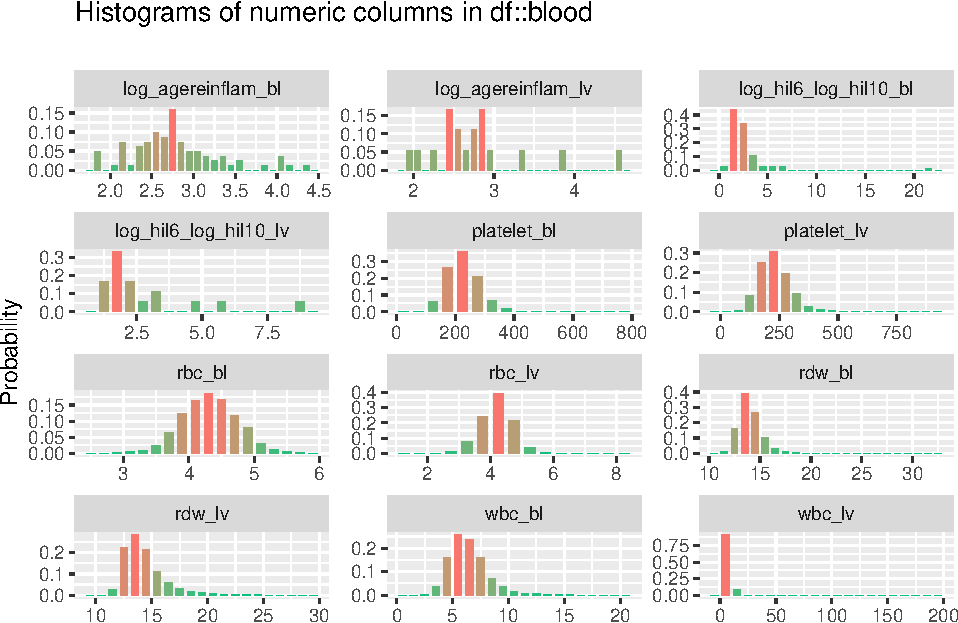
\includegraphics{notebook_files/figure-latex/unnamed-chunk-11-1.pdf}

\hypertarget{htmlwidget-2e3682c30504189c5f2e}{}

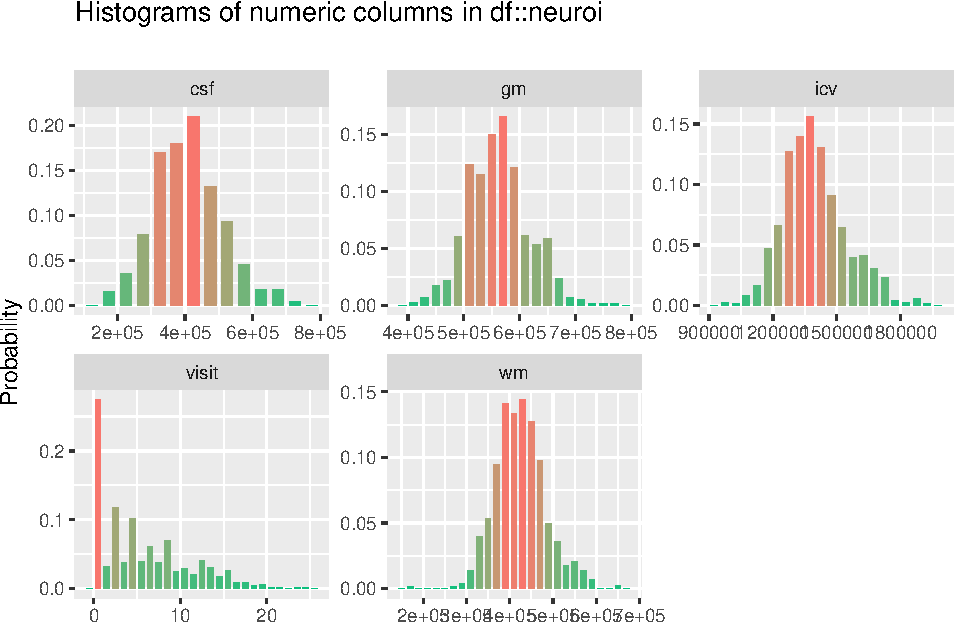
\includegraphics{notebook_files/figure-latex/unnamed-chunk-12-1.pdf}

\hypertarget{cross-tabs-2}{%
\subsection{Cross-tabs}\label{cross-tabs-2}}

\textbf{Characteristic}

0

1

2

3

4

5

6

Unknown

\textbf{Total}

\textbf{ceradsc}

4

10 (2.8\%)

16 (4.4\%)

22 (6.1\%)

16 (4.4\%)

2 (0.6\%)

0 (0\%)

0 (0\%)

2 (0.6\%)

68 (19\%)

3

2 (0.6\%)

2 (0.6\%)

8 (2.2\%)

10 (2.8\%)

3 (0.8\%)

1 (0.3\%)

0 (0\%)

9 (2.5\%)

35 (9.7\%)

2

1 (0.3\%)

15 (4.2\%)

10 (2.8\%)

20 (5.5\%)

11 (3.0\%)

18 (5.0\%)

26 (7.2\%)

8 (2.2\%)

109 (30\%)

1

0 (0\%)

1 (0.3\%)

3 (0.8\%)

13 (3.6\%)

22 (6.1\%)

18 (5.0\%)

81 (22\%)

9 (2.5\%)

147 (41\%)

Unknown

0 (0\%)

0 (0\%)

0 (0\%)

0 (0\%)

1 (0.3\%)

0 (0\%)

0 (0\%)

1 (0.3\%)

2 (0.6\%)

\textbf{Total}

13 (3.6\%)

34 (9.4\%)

43 (12\%)

59 (16\%)

39 (11\%)

37 (10\%)

107 (30\%)

29 (8.0\%)

361 (100\%)

\textbf{Characteristic}

NoAD

Low

Intermediate

High

Unknown

\textbf{Total}

\textbf{cerad}

Normal

10 (2.8\%)

72 (20\%)

3 (0.8\%)

0 (0\%)

13 (3.6\%)

98 (27\%)

Possible

0 (0\%)

26 (7.2\%)

28 (7.8\%)

0 (0\%)

0 (0\%)

54 (15\%)

Probable

0 (0\%)

6 (1.7\%)

31 (8.6\%)

0 (0\%)

4 (1.1\%)

41 (11\%)

Definite

0 (0\%)

4 (1.1\%)

52 (14\%)

99 (27\%)

13 (3.6\%)

168 (47\%)

\textbf{Total}

10 (2.8\%)

108 (30\%)

114 (32\%)

99 (27\%)

30 (8.3\%)

361 (100\%)

\hypertarget{plots-6}{%
\subsection{Plots}\label{plots-6}}

\begin{figure}
\centering
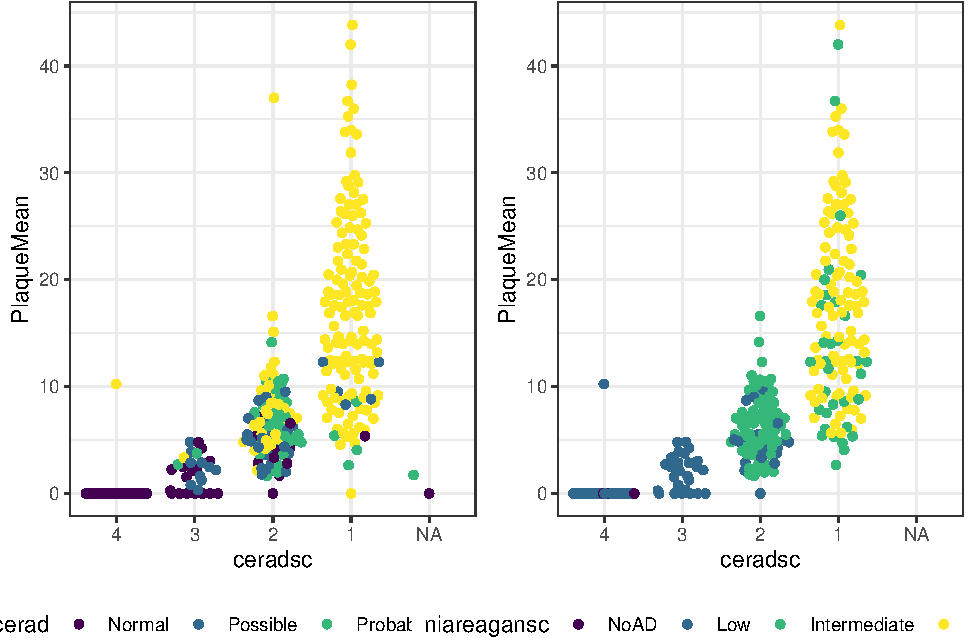
\includegraphics{notebook_files/figure-latex/msbb-plot-plq-cerad-1.pdf}
\caption{\label{fig:msbb-plot-plq-cerad}Distribution of amyloid by neuropathological diagnosis}
\end{figure}

\begin{figure}
\centering
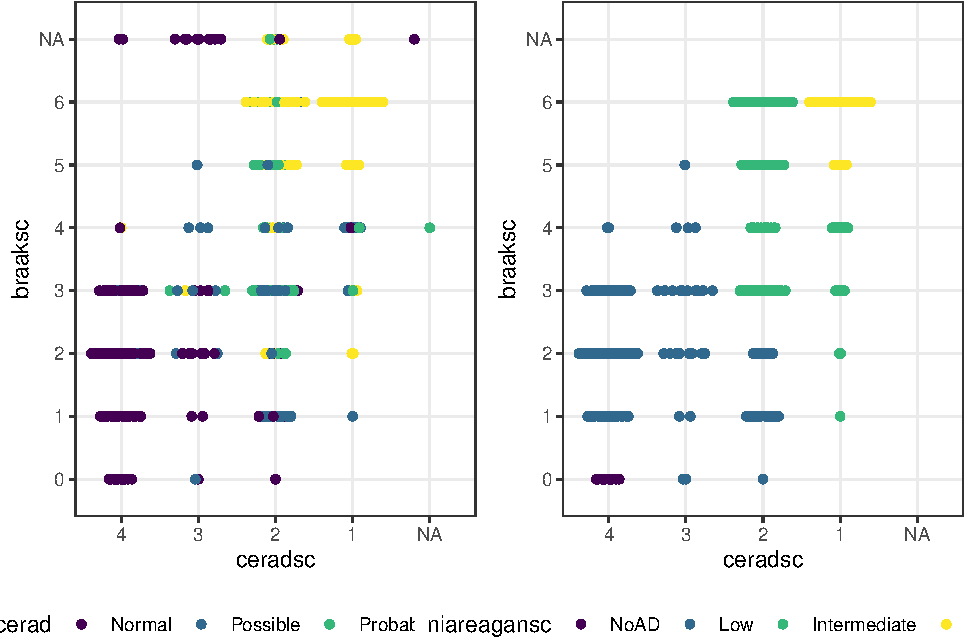
\includegraphics{notebook_files/figure-latex/msbb-plot-plq-braak-1.pdf}
\caption{\label{fig:msbb-plot-plq-braak}Distribution of neuropathological diagnosis by ceradsc and braaksc}
\end{figure}

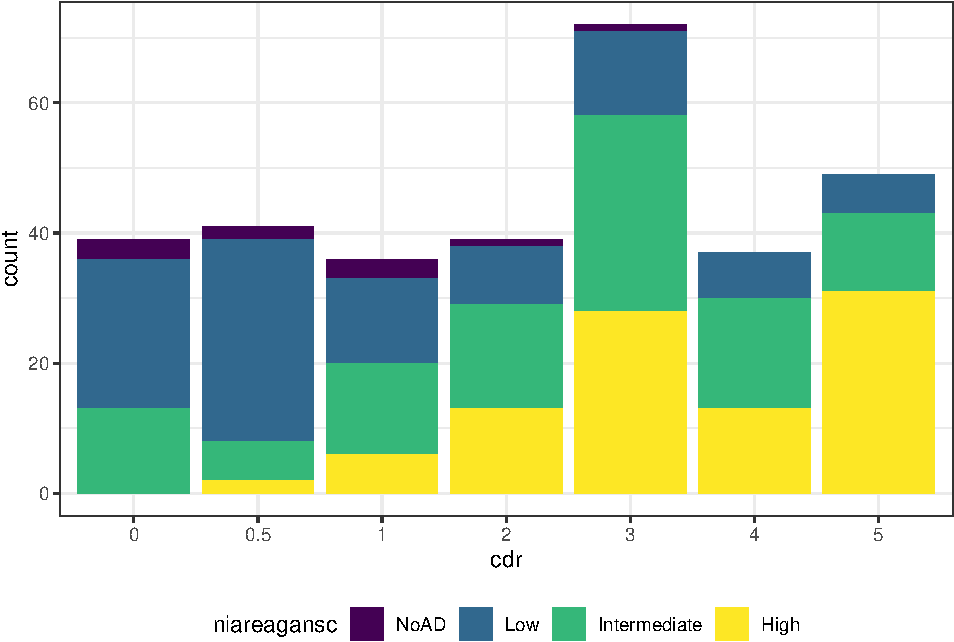
\includegraphics{notebook_files/figure-latex/msbb-plot-cdr-niareagan-1.pdf} 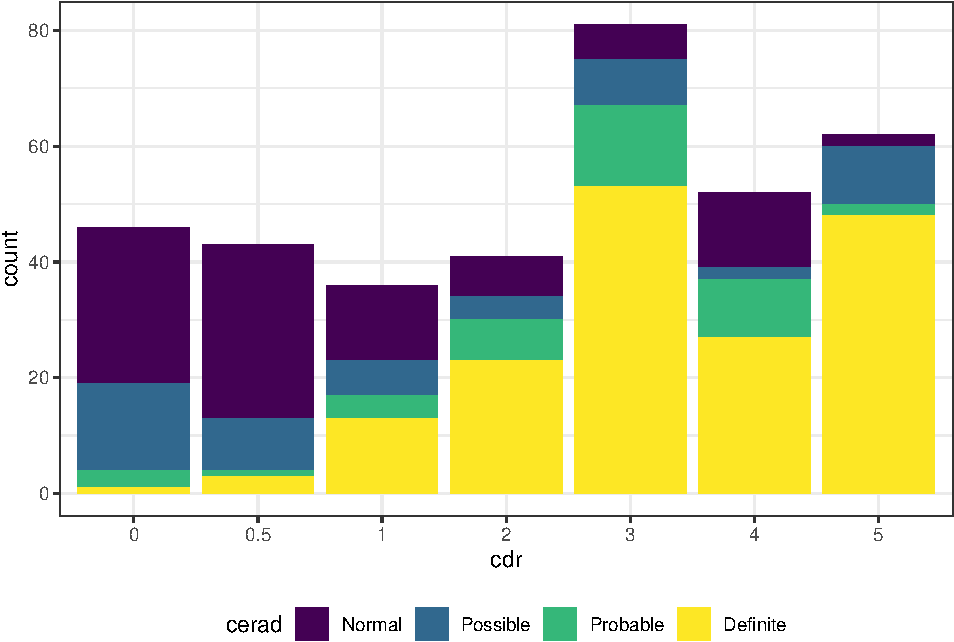
\includegraphics{notebook_files/figure-latex/msbb-plot-cdr-niareagan-2.pdf}

\begin{figure}
\centering
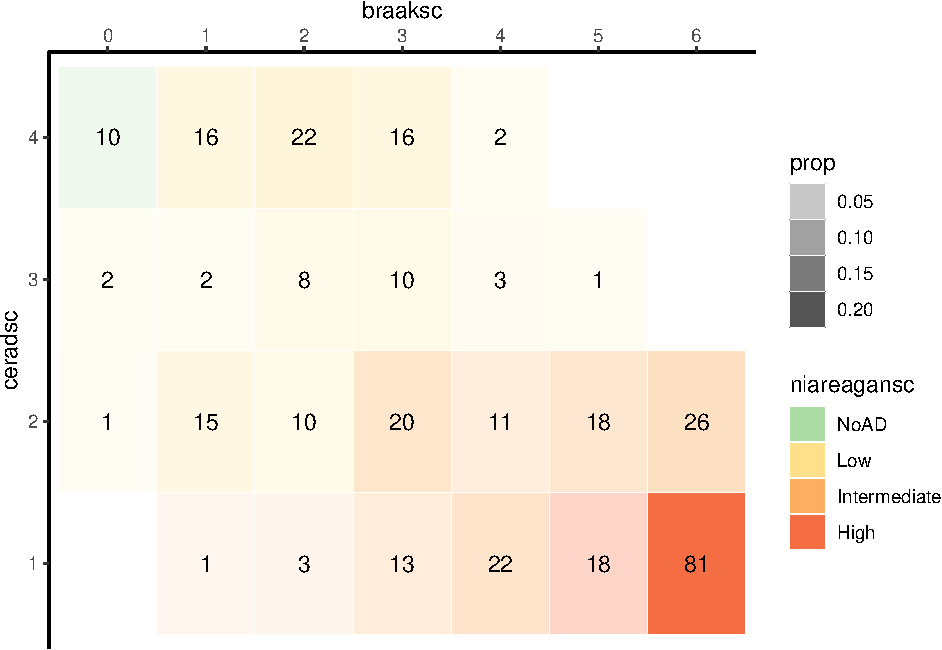
\includegraphics{notebook_files/figure-latex/msbb-plot-cerad-braak-1.pdf}
\caption{\label{fig:msbb-plot-cerad-braak}Cross-tabs of cerad \& braaksc}
\end{figure}

\hypertarget{other-variables}{%
\section{Other Variables}\label{other-variables}}

\label{tab:msbb-numeric}Variable type: Numeric

col\_name

min

q1

median

mean

q3

max

sd

pcnt\_na

PMI

75.00

220.00

315.00

437.21

537.00

1800.00

325.97

0.00

cdr

0.00

1.00

3.00

2.49

4.00

5.00

1.73

0.00

aod

61.00

79.50

85.00

85.09

92.00

108.00

9.37

0.55

mtcn\_avg

734.20

1513.48

1738.74

1726.30

1943.53

3151.59

340.58

0.00

Quality

0.62

0.93

0.96

0.95

0.97

1.01

0.04

0.00

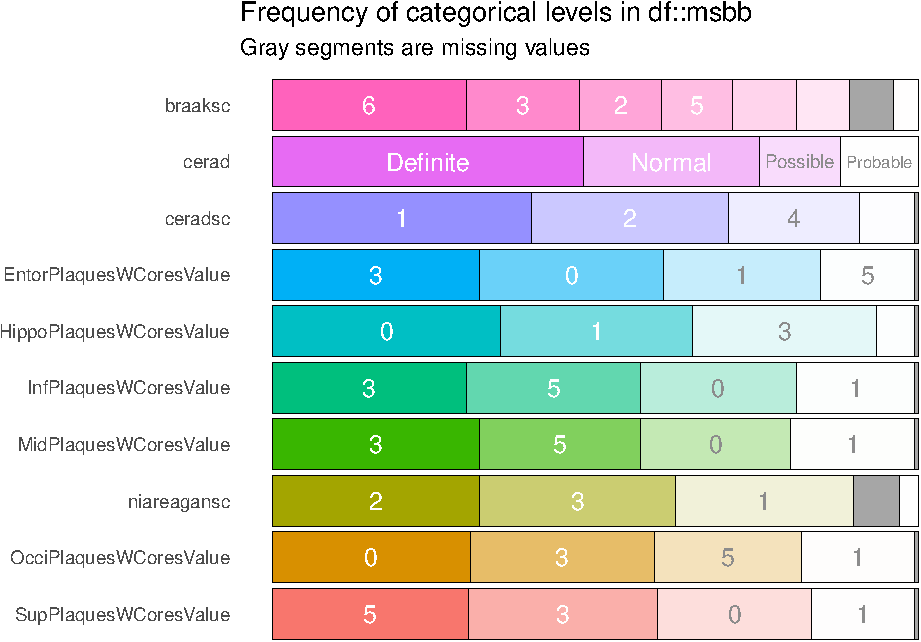
\includegraphics{notebook_files/figure-latex/unnamed-chunk-15-1.pdf}

\hypertarget{htmlwidget-54712731fda672ae3b30}{}

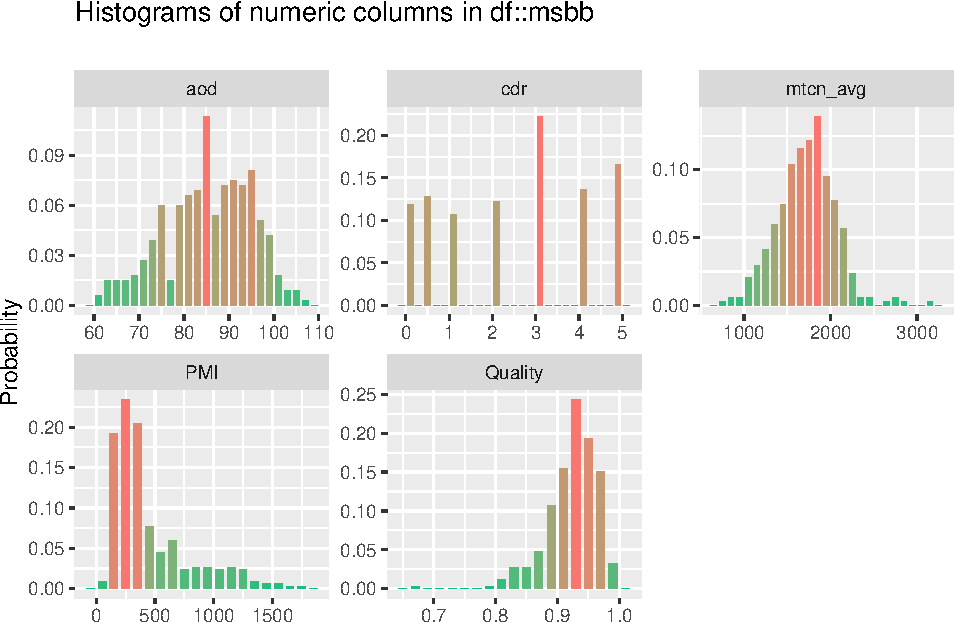
\includegraphics{notebook_files/figure-latex/unnamed-chunk-16-1.pdf}

\hypertarget{mayo}{%
\chapter{MAYO}\label{mayo}}

Allen et al \emph{Human whole genome genotype and transcriptome data for Alzheimer's and other neurodegenerative diseases} \href{https://www.nature.com/articles/sdata201689}{Scientific Data 2016}

Mayo Clinic Alzheimer's Disease Genetics Studies (MCADGS). Data is provided for the Mayo RNAseq Study, with whole transcriptome data for 275 Cerebellum (CBE) and 276 Temporal cortex (TCX) samples from 312 North American Caucasian subjects with neuropathological diagnosis of AD, progressive supranuclear palsy (PSP), pathologic aging (PA) or elderly controls (CON) without neurodegenerative diseases. Whole genome sequencing was conducted on 349 participants using DNA isolated from either the Temporal cortex (n = 341) or the Cerebellar Cortex (n = 8).

\begin{itemize}
\tightlist
\item
  All ADs had definite diagnosis according to the NINCDS-ADRDA criteria and had Braak NFT stage of IV or greater.
\item
  Control subjects had Braak NFT stage of III or less, CERAD neuritic and cortical plaque densities of 0 (none) or 1 (sparse) and lacked any of the following pathologic diagnoses: AD, Parkinson's disease (PD), DLB, VaD, PSP, motor neuron disease (MND), CBD, Pick's disease (PiD), Huntington's disease (HD), FTLD, hippocampal sclerosis (HipScl) or dementia lacking distinctive histology (DLDH).
\item
  Subjects with PA also lacked the above diagnoses and had Braak NFT stage of III or less, but had CERAD neuritic and cortical plaque densities of 2 or more. None of the PA subjects had a clinical diagnosis of dementia or mild cognitive impairment.
\end{itemize}

Clinical Code Book: \href{https://adknowledgeportal.synapse.org/Explore/Studies?Study=syn5550404}{Synapse}

\hypertarget{analysis}{%
\chapter{Analysis}\label{analysis}}

\begin{Shaded}
\begin{Highlighting}[]
\KeywordTok{library}\NormalTok{(tidyverse)}
\KeywordTok{library}\NormalTok{(broom)}
\KeywordTok{library}\NormalTok{(glue)}
\KeywordTok{library}\NormalTok{(ggbeeswarm)}
\KeywordTok{library}\NormalTok{(gvlma)}
\KeywordTok{library}\NormalTok{(inspectdf)}
\NormalTok{knitr}\OperatorTok{::}\NormalTok{opts_knit}\OperatorTok{$}\KeywordTok{set}\NormalTok{(}\DataTypeTok{root.dir =} \StringTok{'/sc/arion/projects/LOAD/shea/Projects/mtDNAcn'}\NormalTok{)}
\end{Highlighting}
\end{Shaded}

\begin{Shaded}
\begin{Highlighting}[]
\NormalTok{rosmap <-}\StringTok{ }\KeywordTok{readRDS}\NormalTok{(}\StringTok{'output/rosmap.RData'}\NormalTok{)}
\NormalTok{msbb <-}\StringTok{ }\KeywordTok{readRDS}\NormalTok{(}\StringTok{'output/msbb.rds'}\NormalTok{)}
\end{Highlighting}
\end{Shaded}

\hypertarget{rosmap-1}{%
\section{ROSMAP}\label{rosmap-1}}

\hypertarget{data-wrangling}{%
\subsection{Data Wrangling}\label{data-wrangling}}

\begin{itemize}
\tightlist
\item
  DNA isolated from Brain tissue

  \begin{itemize}
  \tightlist
  \item
    DLPFC, Posterior Cingulate Cortex, Cerebellum
  \end{itemize}
\item
  European Haplogroups only

  \begin{itemize}
  \tightlist
  \item
    H, V, J, T, U, K, I, W, X
  \end{itemize}
\item
  For clinical diagnosis, exclude MCI, AD possible, other dementia
\end{itemize}

\begin{Shaded}
\begin{Highlighting}[]
\NormalTok{rosmap_df <-}\StringTok{ }\NormalTok{rosmap }\OperatorTok\StringTok{ }
\StringTok{  }\KeywordTok{filter}\NormalTok{(Source.Tissue.Type }\OperatorTok\StringTok{ }\KeywordTok{c}\NormalTok{(}\StringTok{"Brain-DLPFC"}\NormalTok{, }\StringTok{"Brain-Posterior Cingulate Cortex"}\NormalTok{, }\StringTok{"Brain-Cerebellum"}\NormalTok{, }\StringTok{"Whole Blood"}\NormalTok{)) }\OperatorTok
\StringTok{  }\KeywordTok{filter}\NormalTok{(organ }\OperatorTok{==}\StringTok{ 'brain'}\NormalTok{) }\OperatorTok\StringTok{ }
\StringTok{  }\KeywordTok{filter}\NormalTok{(macro }\OperatorTok\StringTok{ }\KeywordTok{c}\NormalTok{(}\StringTok{'H'}\NormalTok{, }\StringTok{'V'}\NormalTok{, }\StringTok{'J'}\NormalTok{, }\StringTok{'T'}\NormalTok{, }\StringTok{'U'}\NormalTok{, }\StringTok{'K'}\NormalTok{, }\StringTok{'I'}\NormalTok{, }\StringTok{'W'}\NormalTok{, }\StringTok{'X'}\NormalTok{)) }\OperatorTok
\StringTok{  }\KeywordTok{filter}\NormalTok{(}\OperatorTok{!}\KeywordTok{is.na}\NormalTok{(macro)) }\OperatorTok
\StringTok{  }\KeywordTok{mutate}\NormalTok{(}\DataTypeTok{ad_reagan =} \KeywordTok{fct_relevel}\NormalTok{(ad_reagan, }\StringTok{"0"}\NormalTok{, }\StringTok{"1"}\NormalTok{),}
         \DataTypeTok{Source.Tissue.Type =} \KeywordTok{fct_inorder}\NormalTok{(Source.Tissue.Type), }
         \DataTypeTok{dx =} \KeywordTok{fct_recode}\NormalTok{(dcfdx_lv, }\StringTok{"0"}\NormalTok{ =}\StringTok{ "1"}\NormalTok{, }\DataTypeTok{NULL =} \StringTok{"2"}\NormalTok{, }\DataTypeTok{NULL =} \StringTok{"3"}\NormalTok{, }\StringTok{"1"}\NormalTok{ =}\StringTok{ "4"}\NormalTok{, }\DataTypeTok{NULL =} \StringTok{"5"}\NormalTok{, }\DataTypeTok{NULL =} \StringTok{"6"}\NormalTok{)) }\OperatorTok
\StringTok{  }\NormalTok{dplyr}\OperatorTok{::}\KeywordTok{select}\NormalTok{(ad_reagan, niareagansc, dcfdx_lv, dx, cts_mmse30_lv, pmi, study, age_death, msex, Source.Tissue.Type, organ, apoe4, z_mtdnacn, macro)}
\end{Highlighting}
\end{Shaded}

\hypertarget{nia-reagan-diagnosis}{%
\subsection{NIA-Reagan Diagnosis}\label{nia-reagan-diagnosis}}

\begin{Shaded}
\begin{Highlighting}[]
\NormalTok{rosmap_path_res <-}\StringTok{ }\KeywordTok{glm}\NormalTok{(ad_reagan }\OperatorTok{~}\StringTok{ }\NormalTok{z_mtdnacn }\OperatorTok{+}\StringTok{ }\NormalTok{macro }\OperatorTok{+}\StringTok{ }\NormalTok{age_death }\OperatorTok{+}\StringTok{ }\NormalTok{msex }\OperatorTok{+}\StringTok{ }\NormalTok{apoe4 }\OperatorTok{+}\StringTok{ }\NormalTok{study }\OperatorTok{+}\StringTok{ }\NormalTok{Source.Tissue.Type, }
                       \DataTypeTok{family =} \StringTok{"binomial"}\NormalTok{, }\DataTypeTok{data =}\NormalTok{ rosmap_df)}
\end{Highlighting}
\end{Shaded}

\label{tab:analysis-rosmap-path-tab}Assocation of mtDNA with MMSE in ROSMAP

term

estimate

std.error

statistic

p.value

(Intercept)

-5.864

1.256

-4.670

3.0e-06 ***

z\_mtdnacn

-0.458

0.197

-2.320

0.02 *

macroI

-0.031

0.455

-0.068

0.946

macroJ

0.697

0.337

2.071

0.038 *

macroK

0.111

0.327

0.340

0.734

macroT

0.153

0.289

0.529

0.597

macroU

0.015

0.238

0.064

0.949

macroV

0.344

0.405

0.850

0.396

macroW

-0.087

0.634

-0.138

0.89

macroX

0.368

0.717

0.514

0.608

age\_death

0.076

0.013

5.624

1.9e-08 ***

msexM

-0.330

0.175

-1.887

0.059 .

apoe4e4+

1.416

0.223

6.357

2.1e-10 ***

studyROS

0.050

0.171

0.294

0.768

Source.Tissue.TypeBrain-Cerebellum

-1.013

0.348

-2.909

0.004 **

Source.Tissue.TypeBrain-Posterior Cingulate Cortex

-0.076

0.304

-0.250

0.802

\begin{Shaded}
\begin{Highlighting}[]
\KeywordTok{ggplot}\NormalTok{(rosmap_df, }\KeywordTok{aes}\NormalTok{(}\DataTypeTok{x =}\NormalTok{ ad_reagan, }\DataTypeTok{y =}\NormalTok{ z_mtdnacn, }\DataTypeTok{colour =}\NormalTok{ Source.Tissue.Type)) }\OperatorTok{+}\StringTok{ }
\StringTok{  }\KeywordTok{geom_quasirandom}\NormalTok{() }\OperatorTok{+}\StringTok{ }
\StringTok{  }\KeywordTok{geom_pointrange}\NormalTok{(}\DataTypeTok{mapping =} \KeywordTok{aes}\NormalTok{(}\DataTypeTok{x =}\NormalTok{ ad_reagan, }\DataTypeTok{y =}\NormalTok{ z_mtdnacn),}
                      \DataTypeTok{show.legend =}\NormalTok{ F, }\DataTypeTok{colour =} \StringTok{'black'}\NormalTok{,}
                     \CommentTok{# size = 1,}
                      \DataTypeTok{position =} \KeywordTok{position_dodge}\NormalTok{(}\DataTypeTok{width =} \DecValTok{1}\NormalTok{),}
                      \DataTypeTok{shape =} \DecValTok{15}\NormalTok{,}
                      \DataTypeTok{stat =} \StringTok{"summary"}\NormalTok{,}
                      \DataTypeTok{fun =}\NormalTok{ median,}
                      \DataTypeTok{fun.min =} \ControlFlowTok{function}\NormalTok{(z) \{}\KeywordTok{quantile}\NormalTok{(z,}\FloatTok{0.25}\NormalTok{)\},}
                      \DataTypeTok{fun.max =} \ControlFlowTok{function}\NormalTok{(z) \{}\KeywordTok{quantile}\NormalTok{(z,}\FloatTok{0.75}\NormalTok{)\}) }\OperatorTok{+}\StringTok{ }
\StringTok{  }\KeywordTok{theme_bw}\NormalTok{() }\OperatorTok{+}\StringTok{ }\KeywordTok{theme}\NormalTok{(}\DataTypeTok{legend.position =} \StringTok{"bottom"}\NormalTok{)}
\end{Highlighting}
\end{Shaded}

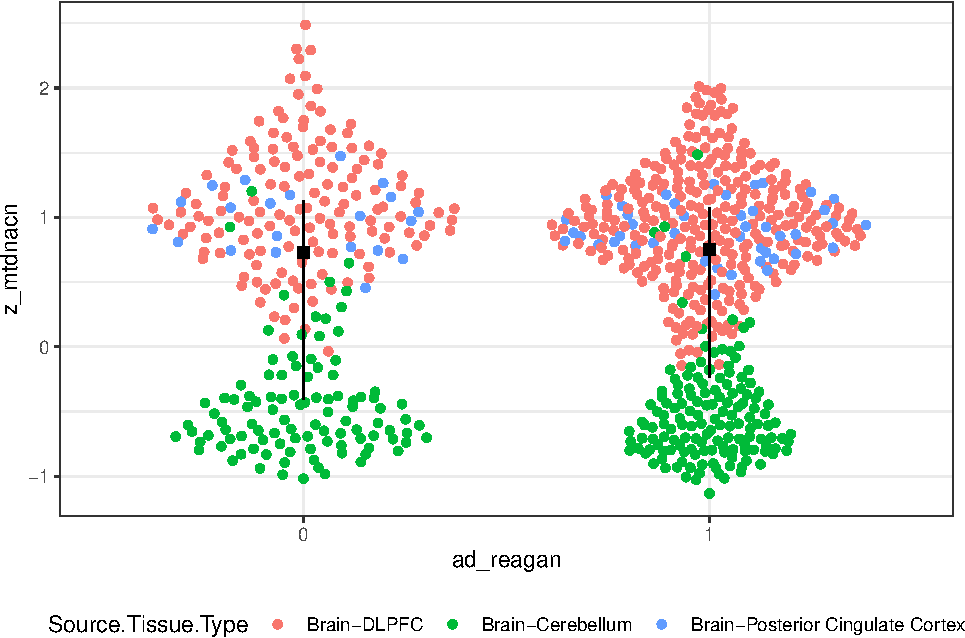
\includegraphics{notebook_files/figure-latex/analysis-rosmap-path-plot-1.pdf}

\hypertarget{clinical-diagnosis-1}{%
\subsection{Clinical diagnosis}\label{clinical-diagnosis-1}}

\begin{Shaded}
\begin{Highlighting}[]
\NormalTok{rosmap_clin_res <-}\StringTok{ }\KeywordTok{glm}\NormalTok{(dx }\OperatorTok{~}\StringTok{ }\NormalTok{z_mtdnacn }\OperatorTok{+}\StringTok{ }\NormalTok{macro }\OperatorTok{+}\StringTok{ }\NormalTok{age_death }\OperatorTok{+}\StringTok{ }\NormalTok{msex }\OperatorTok{+}\StringTok{ }\NormalTok{apoe4 }\OperatorTok{+}\StringTok{ }\NormalTok{study }\OperatorTok{+}\StringTok{ }\NormalTok{Source.Tissue.Type, }\DataTypeTok{family =} \StringTok{"binomial"}\NormalTok{, }\DataTypeTok{data =}\NormalTok{ rosmap_df)}
\end{Highlighting}
\end{Shaded}

\label{tab:analysis-rosmap-clin-tab}Assocation of mtDNA with MMSE in ROSMAP

term

estimate

std.error

statistic

p.value

(Intercept)

-9.890

1.591

-6.215

5.1e-10 ***

z\_mtdnacn

-0.453

0.248

-1.829

0.067 .

macroI

0.340

0.596

0.571

0.568

macroJ

0.092

0.396

0.233

0.816

macroK

0.991

0.437

2.266

0.023 *

macroT

-0.030

0.333

-0.091

0.928

macroU

0.340

0.283

1.202

0.23

macroV

0.502

0.483

1.039

0.299

macroW

0.595

0.733

0.812

0.417

macroX

-0.590

0.734

-0.804

0.421

age\_death

0.110

0.017

6.479

9.3e-11 ***

msexM

-0.081

0.213

-0.379

0.704

apoe4e4+

1.429

0.243

5.881

4.1e-09 ***

studyROS

0.275

0.208

1.322

0.186

Source.Tissue.TypeBrain-Cerebellum

-0.426

0.417

-1.023

0.306

Source.Tissue.TypeBrain-Posterior Cingulate Cortex

0.003

0.360

0.008

0.994

\begin{Shaded}
\begin{Highlighting}[]
\NormalTok{rosmap_df }\OperatorTok\StringTok{ }
\StringTok{  }\KeywordTok{filter}\NormalTok{(}\OperatorTok{!}\KeywordTok{is.na}\NormalTok{(dx)) }\OperatorTok
\StringTok{  }\KeywordTok{ggplot}\NormalTok{(., }\KeywordTok{aes}\NormalTok{(}\DataTypeTok{x =}\NormalTok{ dx, }\DataTypeTok{y =}\NormalTok{ z_mtdnacn, }\DataTypeTok{colour =}\NormalTok{ Source.Tissue.Type)) }\OperatorTok{+}\StringTok{ }
\StringTok{    }\KeywordTok{geom_quasirandom}\NormalTok{() }\OperatorTok{+}\StringTok{ }
\StringTok{    }\KeywordTok{geom_pointrange}\NormalTok{(}\DataTypeTok{mapping =} \KeywordTok{aes}\NormalTok{(}\DataTypeTok{x =}\NormalTok{ dx, }\DataTypeTok{y =}\NormalTok{ z_mtdnacn),}
                        \DataTypeTok{show.legend =}\NormalTok{ F, }\DataTypeTok{colour =} \StringTok{'black'}\NormalTok{,}
                       \CommentTok{# size = 1,}
                        \DataTypeTok{position =} \KeywordTok{position_dodge}\NormalTok{(}\DataTypeTok{width =} \DecValTok{1}\NormalTok{),}
                        \DataTypeTok{shape =} \DecValTok{15}\NormalTok{,}
                        \DataTypeTok{stat =} \StringTok{"summary"}\NormalTok{,}
                        \DataTypeTok{fun =}\NormalTok{ median,}
                        \DataTypeTok{fun.min =} \ControlFlowTok{function}\NormalTok{(z) \{}\KeywordTok{quantile}\NormalTok{(z,}\FloatTok{0.25}\NormalTok{)\},}
                        \DataTypeTok{fun.max =} \ControlFlowTok{function}\NormalTok{(z) \{}\KeywordTok{quantile}\NormalTok{(z,}\FloatTok{0.75}\NormalTok{)\}) }\OperatorTok{+}\StringTok{ }
\StringTok{  }\KeywordTok{theme_bw}\NormalTok{() }\OperatorTok{+}\StringTok{ }\KeywordTok{theme}\NormalTok{(}\DataTypeTok{legend.position =} \StringTok{"bottom"}\NormalTok{)}
\end{Highlighting}
\end{Shaded}

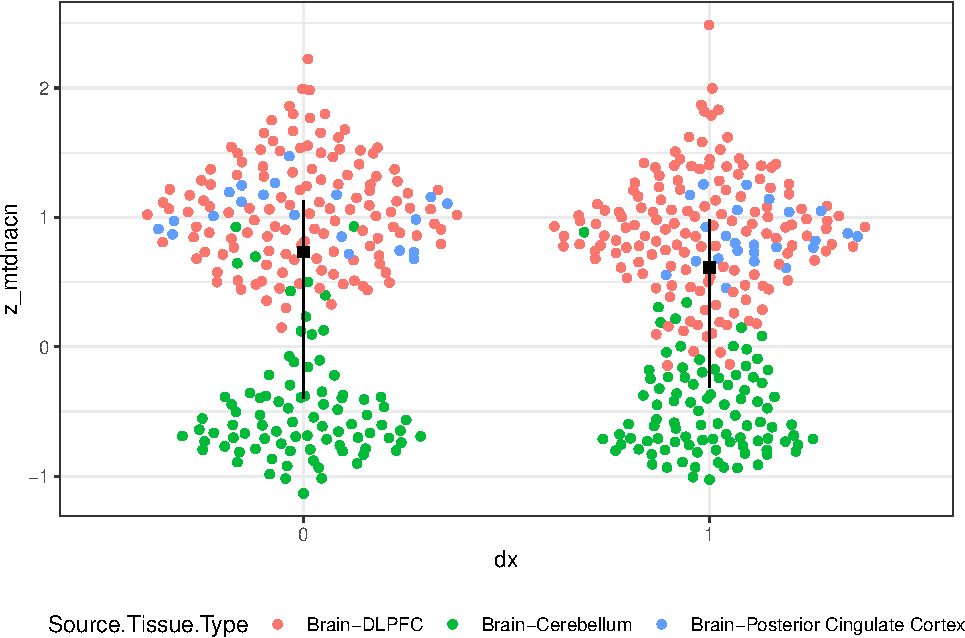
\includegraphics{notebook_files/figure-latex/clin-plot-1.pdf}

\hypertarget{msbb-1}{%
\section{MSBB}\label{msbb-1}}

\hypertarget{data-wrangling-1}{%
\subsection{Data Wrangling}\label{data-wrangling-1}}

\begin{itemize}
\tightlist
\item
  Exclude individules who are not non-hispanic whites
\item
  Exclude individules with non-European haplogroups
\item
  Dichotomize CERAD dx
\end{itemize}

\begin{Shaded}
\begin{Highlighting}[]
\NormalTok{msbb_df <-}\StringTok{ }\NormalTok{msbb  }\OperatorTok\StringTok{ }
\StringTok{  }\KeywordTok{filter}\NormalTok{(race }\OperatorTok{==}\StringTok{ 'W'}\NormalTok{) }\OperatorTok
\StringTok{  }\KeywordTok{filter}\NormalTok{(macro }\OperatorTok\StringTok{ }\KeywordTok{c}\NormalTok{(}\StringTok{'H'}\NormalTok{, }\StringTok{'V'}\NormalTok{, }\StringTok{'J'}\NormalTok{, }\StringTok{'T'}\NormalTok{, }\StringTok{'U'}\NormalTok{, }\StringTok{'K'}\NormalTok{, }\StringTok{'I'}\NormalTok{, }\StringTok{'W'}\NormalTok{, }\StringTok{'X'}\NormalTok{)) }\OperatorTok\StringTok{ }
\StringTok{  }\KeywordTok{mutate}\NormalTok{(}\DataTypeTok{cerad_dx =} \KeywordTok{fct_recode}\NormalTok{(cerad, }\StringTok{"0"}\NormalTok{ =}\StringTok{ "Normal"}\NormalTok{, }\StringTok{"0"}\NormalTok{ =}\StringTok{ "Possible"}\NormalTok{, }\StringTok{"1"}\NormalTok{ =}\StringTok{ "Probable"}\NormalTok{, }\StringTok{"1"}\NormalTok{ =}\StringTok{ "Definite"}\NormalTok{))}
\end{Highlighting}
\end{Shaded}

\hypertarget{nia-reagan}{%
\subsection{NIA-Reagan}\label{nia-reagan}}

\begin{Shaded}
\begin{Highlighting}[]
\NormalTok{msbb_path_res <-}\StringTok{ }\KeywordTok{glm}\NormalTok{(ad_reagan }\OperatorTok{~}\StringTok{ }\NormalTok{z_mtdnacn }\OperatorTok{+}\StringTok{ }\NormalTok{macro }\OperatorTok{+}\StringTok{ }\NormalTok{aod }\OperatorTok{+}\StringTok{ }\NormalTok{sex }\OperatorTok{+}\StringTok{ }\NormalTok{apoe4, }
                       \DataTypeTok{family =} \StringTok{"binomial"}\NormalTok{, }\DataTypeTok{data =}\NormalTok{ msbb_df)}
\end{Highlighting}
\end{Shaded}

\label{tab:analysis-msbb-path-tab}Assocation of mtDNA with MMSE in msbb

term

estimate

std.error

statistic

p.value

(Intercept)

-2.204

1.542

-1.430

0.153

z\_mtdnacn

-0.268

0.146

-1.837

0.066 .

macroI

15.877

1684.913

0.009

0.992

macroJ

0.088

0.498

0.177

0.86

macroK

0.342

0.372

0.920

0.358

macroT

0.866

0.630

1.374

0.169

macroU

0.767

0.561

1.367

0.172

macroV

0.936

0.615

1.522

0.128

macroW

16.010

1357.213

0.012

0.991

macroX

-0.201

1.040

-0.193

0.847

aod

0.026

0.017

1.517

0.129

sexM

0.411

0.341

1.206

0.228

apoe4e4+

0.760

0.320

2.375

0.018 *

\begin{Shaded}
\begin{Highlighting}[]
\NormalTok{msbb_df }\OperatorTok\StringTok{ }
\StringTok{  }\KeywordTok{filter}\NormalTok{(}\OperatorTok{!}\KeywordTok{is.na}\NormalTok{(ad_reagan)) }\OperatorTok
\StringTok{    }\KeywordTok{ggplot}\NormalTok{(., }\KeywordTok{aes}\NormalTok{(}\DataTypeTok{x =}\NormalTok{ ad_reagan, }\DataTypeTok{y =}\NormalTok{ z_mtdnacn, }\DataTypeTok{colour =}\NormalTok{ ad_reagan)) }\OperatorTok{+}\StringTok{ }
\StringTok{      }\KeywordTok{geom_quasirandom}\NormalTok{() }\OperatorTok{+}\StringTok{ }
\StringTok{      }\KeywordTok{geom_pointrange}\NormalTok{(}\DataTypeTok{mapping =} \KeywordTok{aes}\NormalTok{(}\DataTypeTok{x =}\NormalTok{ ad_reagan, }\DataTypeTok{y =}\NormalTok{ z_mtdnacn),}
                          \DataTypeTok{show.legend =}\NormalTok{ F, }\DataTypeTok{colour =} \StringTok{'black'}\NormalTok{,}
                         \CommentTok{# size = 1,}
                          \DataTypeTok{position =} \KeywordTok{position_dodge}\NormalTok{(}\DataTypeTok{width =} \DecValTok{1}\NormalTok{),}
                          \DataTypeTok{shape =} \DecValTok{15}\NormalTok{,}
                          \DataTypeTok{stat =} \StringTok{"summary"}\NormalTok{,}
                          \DataTypeTok{fun =}\NormalTok{ median,}
                          \DataTypeTok{fun.min =} \ControlFlowTok{function}\NormalTok{(z) \{}\KeywordTok{quantile}\NormalTok{(z,}\FloatTok{0.25}\NormalTok{)\},}
                          \DataTypeTok{fun.max =} \ControlFlowTok{function}\NormalTok{(z) \{}\KeywordTok{quantile}\NormalTok{(z,}\FloatTok{0.75}\NormalTok{)\}) }\OperatorTok{+}\StringTok{ }
\StringTok{      }\KeywordTok{theme_bw}\NormalTok{() }\OperatorTok{+}\StringTok{ }\KeywordTok{theme}\NormalTok{(}\DataTypeTok{legend.position =} \StringTok{"bottom"}\NormalTok{)}
\end{Highlighting}
\end{Shaded}

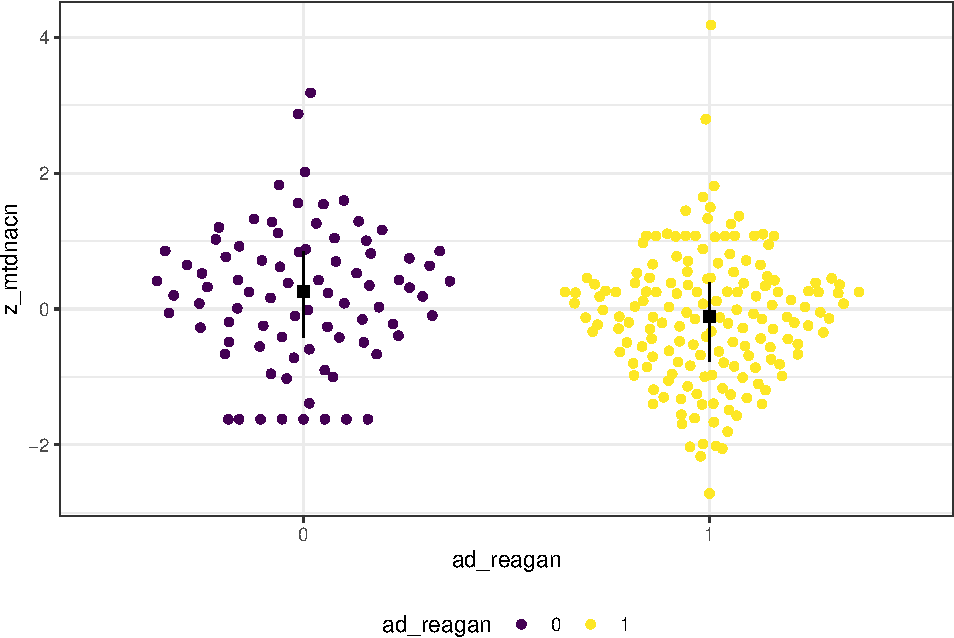
\includegraphics{notebook_files/figure-latex/analysis-msbb-path-plot-1.pdf}

\hypertarget{cerad}{%
\subsection{CERAD}\label{cerad}}

\begin{Shaded}
\begin{Highlighting}[]
\NormalTok{msbb_cerad_res <-}\StringTok{ }\KeywordTok{glm}\NormalTok{(cerad_dx }\OperatorTok{~}\StringTok{ }\NormalTok{z_mtdnacn }\OperatorTok{+}\StringTok{ }\NormalTok{macro }\OperatorTok{+}\StringTok{ }\NormalTok{aod }\OperatorTok{+}\StringTok{ }\NormalTok{sex }\OperatorTok{+}\StringTok{ }\NormalTok{apoe4, }
                       \DataTypeTok{family =} \StringTok{"binomial"}\NormalTok{, }\DataTypeTok{data =}\NormalTok{ msbb_df)}
\end{Highlighting}
\end{Shaded}

\label{tab:analysis-msbb-cerad-tab}Assocation of mtDNA with MMSE in msbb

term

estimate

std.error

statistic

p.value

(Intercept)

-1.680

1.500

-1.120

0.263

z\_mtdnacn

-0.629

0.151

-4.155

3.3e-05 ***

macroI

15.049

840.116

0.018

0.986

macroJ

-0.182

0.419

-0.434

0.664

macroK

0.748

0.359

2.081

0.037 *

macroT

0.934

0.597

1.564

0.118

macroU

2.208

0.782

2.825

0.005 **

macroV

1.002

0.576

1.740

0.082 .

macroW

0.854

1.261

0.677

0.498

macroX

0.252

1.026

0.246

0.806

aod

0.017

0.017

1.028

0.304

sexM

0.338

0.312

1.082

0.279

apoe4e4+

0.358

0.291

1.233

0.217

\begin{Shaded}
\begin{Highlighting}[]
\NormalTok{msbb_df }\OperatorTok\StringTok{ }
\StringTok{  }\KeywordTok{filter}\NormalTok{(}\OperatorTok{!}\KeywordTok{is.na}\NormalTok{(cerad_dx)) }\OperatorTok
\StringTok{    }\KeywordTok{ggplot}\NormalTok{(., }\KeywordTok{aes}\NormalTok{(}\DataTypeTok{x =}\NormalTok{ cerad_dx, }\DataTypeTok{y =}\NormalTok{ z_mtdnacn, }\DataTypeTok{colour =}\NormalTok{ cerad_dx)) }\OperatorTok{+}\StringTok{ }
\StringTok{      }\KeywordTok{geom_quasirandom}\NormalTok{() }\OperatorTok{+}\StringTok{ }
\StringTok{      }\KeywordTok{geom_pointrange}\NormalTok{(}\DataTypeTok{mapping =} \KeywordTok{aes}\NormalTok{(}\DataTypeTok{x =}\NormalTok{ cerad_dx, }\DataTypeTok{y =}\NormalTok{ z_mtdnacn),}
                          \DataTypeTok{show.legend =}\NormalTok{ F, }\DataTypeTok{colour =} \StringTok{'black'}\NormalTok{,}
                         \CommentTok{# size = 1,}
                          \DataTypeTok{position =} \KeywordTok{position_dodge}\NormalTok{(}\DataTypeTok{width =} \DecValTok{1}\NormalTok{),}
                          \DataTypeTok{shape =} \DecValTok{15}\NormalTok{,}
                          \DataTypeTok{stat =} \StringTok{"summary"}\NormalTok{,}
                          \DataTypeTok{fun =}\NormalTok{ median,}
                          \DataTypeTok{fun.min =} \ControlFlowTok{function}\NormalTok{(z) \{}\KeywordTok{quantile}\NormalTok{(z,}\FloatTok{0.25}\NormalTok{)\},}
                          \DataTypeTok{fun.max =} \ControlFlowTok{function}\NormalTok{(z) \{}\KeywordTok{quantile}\NormalTok{(z,}\FloatTok{0.75}\NormalTok{)\}) }\OperatorTok{+}\StringTok{ }
\StringTok{      }\KeywordTok{theme_bw}\NormalTok{() }\OperatorTok{+}\StringTok{ }\KeywordTok{theme}\NormalTok{(}\DataTypeTok{legend.position =} \StringTok{"bottom"}\NormalTok{)}
\end{Highlighting}
\end{Shaded}

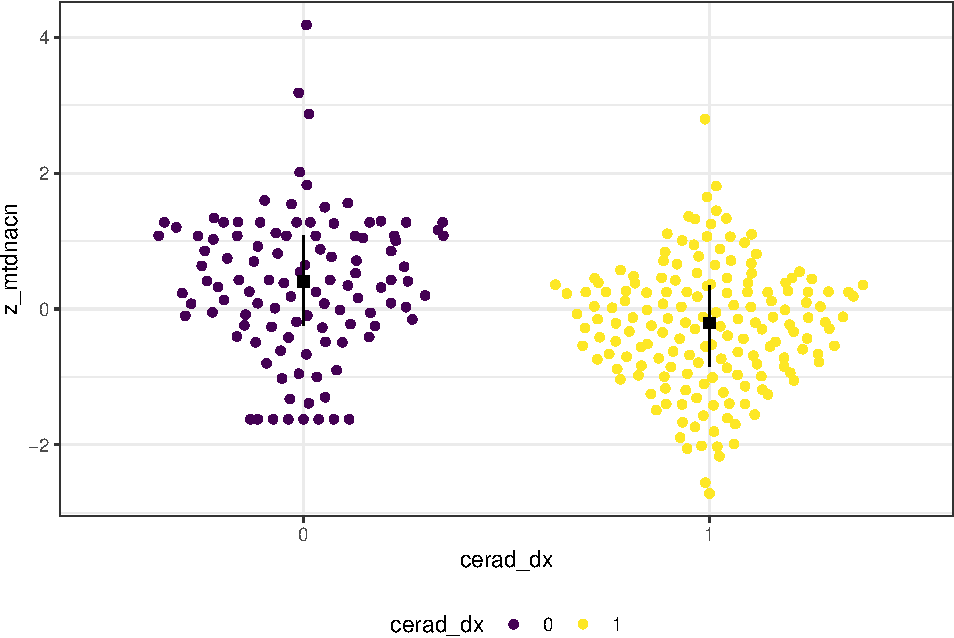
\includegraphics{notebook_files/figure-latex/analysis-msbb-cerad-plot-1.pdf}

\hypertarget{aaic-abstract}{%
\chapter{AAIC Abstract}\label{aaic-abstract}}

\textbf{Mitochondrial DNA copy number is associated with cognitive impairment}

\textbf{Background:} Increasing evidence has implicated mitochondrial dysfunction in the pathogenesis of Alzheimer's Disease. Mitochondria contain their own DNA outside of the nuclear genome, with every cell having between 100-10,000 copies of mtDNA. Mitochondrial DNA copy number (mtDNA-CN) has been used as a surrogate measure of mitochondrial function, with reduced mtDNA-CN associated with age-related diseases. The aim of this study was to evaluate the association of mtDNA-CN with cognitive impairment.

\begin{Shaded}
\begin{Highlighting}[]
\NormalTok{rosmap.raw  <-}\StringTok{ }\KeywordTok{readRDS}\NormalTok{(}\StringTok{'output/rosmap.RData'}\NormalTok{) }
\NormalTok{rosmap <-}\StringTok{ }\NormalTok{rosmap.raw }\OperatorTok\StringTok{ }
\StringTok{  }\KeywordTok{filter}\NormalTok{(Source.Tissue.Type }\OperatorTok\StringTok{ }\KeywordTok{c}\NormalTok{(}\StringTok{"Brain-DLPFC"}\NormalTok{, }\StringTok{"Brain-Posterior Cingulate Cortex"}\NormalTok{, }\StringTok{"Brain-Cerebellum"}\NormalTok{, }\StringTok{"Whole Blood"}\NormalTok{)) }\OperatorTok
\StringTok{  }\KeywordTok{filter}\NormalTok{(organ }\OperatorTok{==}\StringTok{ 'brain'}\NormalTok{) }\OperatorTok\StringTok{ }
\StringTok{  }\KeywordTok{filter}\NormalTok{(macro }\OperatorTok\StringTok{ }\KeywordTok{c}\NormalTok{(}\StringTok{'H'}\NormalTok{, }\StringTok{'V'}\NormalTok{, }\StringTok{'J'}\NormalTok{, }\StringTok{'T'}\NormalTok{, }\StringTok{'U'}\NormalTok{, }\StringTok{'K'}\NormalTok{, }\StringTok{'I'}\NormalTok{, }\StringTok{'W'}\NormalTok{, }\StringTok{'X'}\NormalTok{)) }\OperatorTok
\StringTok{  }\KeywordTok{filter}\NormalTok{(}\OperatorTok{!}\KeywordTok{is.na}\NormalTok{(macro)) }\OperatorTok
\StringTok{  }\KeywordTok{filter}\NormalTok{(}\OperatorTok{!}\KeywordTok{is.na}\NormalTok{(cts_mmse30_lv)) }\OperatorTok
\StringTok{  }\KeywordTok{filter}\NormalTok{(}\OperatorTok{!}\KeywordTok{is.na}\NormalTok{(apoe4)) }\OperatorTok\StringTok{ }
\StringTok{  }\KeywordTok{mutate}\NormalTok{(}\DataTypeTok{Source.Tissue.Type =} \KeywordTok{str_replace}\NormalTok{(Source.Tissue.Type, }\StringTok{"Brain-"}\NormalTok{, }\StringTok{""}\NormalTok{), }
         \DataTypeTok{Source.Tissue.Type =} \KeywordTok{str_replace}\NormalTok{(Source.Tissue.Type, }\StringTok{"Posterior Cingulate Cortex"}\NormalTok{, }\StringTok{"PCC"}\NormalTok{)) }\OperatorTok
\StringTok{  }\KeywordTok{select}\NormalTok{(cts_mmse30_lv, niareagansc, dcfdx_lv, cts_mmse30_lv, pmi, study, age_death, msex, }
\NormalTok{         Source.Tissue.Type, organ, apoe4, z_mtdnacn, mtcn_avg, macro)}
\end{Highlighting}
\end{Shaded}

\begin{Shaded}
\begin{Highlighting}[]
\NormalTok{msbb.raw <-}\StringTok{ }\KeywordTok{readRDS}\NormalTok{(}\StringTok{'output/msbb.rds'}\NormalTok{)}

\NormalTok{msbb <-}\StringTok{ }\NormalTok{msbb.raw  }\OperatorTok\StringTok{ }
\StringTok{  }\KeywordTok{filter}\NormalTok{(race }\OperatorTok{==}\StringTok{ 'W'}\NormalTok{) }\OperatorTok
\StringTok{  }\KeywordTok{filter}\NormalTok{(macro }\OperatorTok\StringTok{ }\KeywordTok{c}\NormalTok{(}\StringTok{'H'}\NormalTok{, }\StringTok{'V'}\NormalTok{, }\StringTok{'J'}\NormalTok{, }\StringTok{'T'}\NormalTok{, }\StringTok{'U'}\NormalTok{, }\StringTok{'K'}\NormalTok{, }\StringTok{'I'}\NormalTok{, }\StringTok{'W'}\NormalTok{, }\StringTok{'X'}\NormalTok{)) }
\end{Highlighting}
\end{Shaded}

\textbf{Methods:} We evaluated the association of mtDNA-CN with the extended Clinical Dementia Rating (CDR) scale in the Mount Sinai Brain Bank (MSBB) and with mini mental state exam (MMSE) in the Religious Orders Studies and the Memory Aging Project (ROSMAP). Relative mtDNA-CN was estimated as the ratio of mitochondrial genomes to nuclear genomes in 1025 non-Hispanic white subjects (MSBB = 277; ROSMAP = 748) using whole-genome sequencing data generated from DNA isolated from post-mortem brain tissue (MSBB: prefrontal cortex; ROSMAP: dorsolateral prefrontal cortex {[}DLPFC{]}, posterior cingulate cortex {[}PCC{]}, or cerebellum). Linear regression adjusting for age of death, sex, APOE, study, mitochondrial haplogroup and source tissue were used to evaluate the association of mtDNA-CN with cognitive impairment.

\begin{Shaded}
\begin{Highlighting}[]
\CommentTok{## CDR analysis}
\NormalTok{cdr_res <-}\StringTok{ }\KeywordTok{lm}\NormalTok{(cdr }\OperatorTok{~}\StringTok{ }\NormalTok{z_mtdnacn  }\OperatorTok{+}\StringTok{ }\NormalTok{aod }\OperatorTok{+}\StringTok{ }\NormalTok{sex }\OperatorTok{+}\StringTok{ }\NormalTok{apoe4 }\OperatorTok{+}\StringTok{ }\NormalTok{macro, }\DataTypeTok{data =}\NormalTok{ msbb)}
\NormalTok{cdr_tab <-}\StringTok{ }\KeywordTok{tidy}\NormalTok{(cdr_res)}

\CommentTok{## MMSE analysis}
\NormalTok{mmse_res <-}\StringTok{ }\KeywordTok{lm}\NormalTok{(cts_mmse30_lv }\OperatorTok{~}\StringTok{ }\NormalTok{z_mtdnacn  }\OperatorTok{+}\StringTok{ }\NormalTok{age_death }\OperatorTok{+}\StringTok{ }\NormalTok{msex }\OperatorTok{+}\StringTok{ }\NormalTok{apoe4 }\OperatorTok{+}\StringTok{ }\NormalTok{study }\OperatorTok{+}\StringTok{ }\NormalTok{Source.Tissue.Type }\OperatorTok{+}\StringTok{ }\NormalTok{macro, }\DataTypeTok{data =}\NormalTok{ rosmap)}
\NormalTok{mmse_tab <-}\StringTok{ }\KeywordTok{tidy}\NormalTok{(mmse_res)}
\end{Highlighting}
\end{Shaded}

\textbf{Results:} In the MSBB, a one standard deviation decrease (1 s.d. 343) in mtDNA-CN was associated with a higher CDR score (\(\beta\)(se) = 0.7 (0.1), p = 3.41e-12, \ref{print-aaic-plots}). Similarly, in ROSMAP a one standard deviation decrease (1 s.d. 1063) in mtDNA-CN was associated with a lower MMSE score (\(\beta\)(se) = -4.02 (0.75), p = 1.07e-07, \ref{print-aaic-plots}).

\begin{figure}
\centering
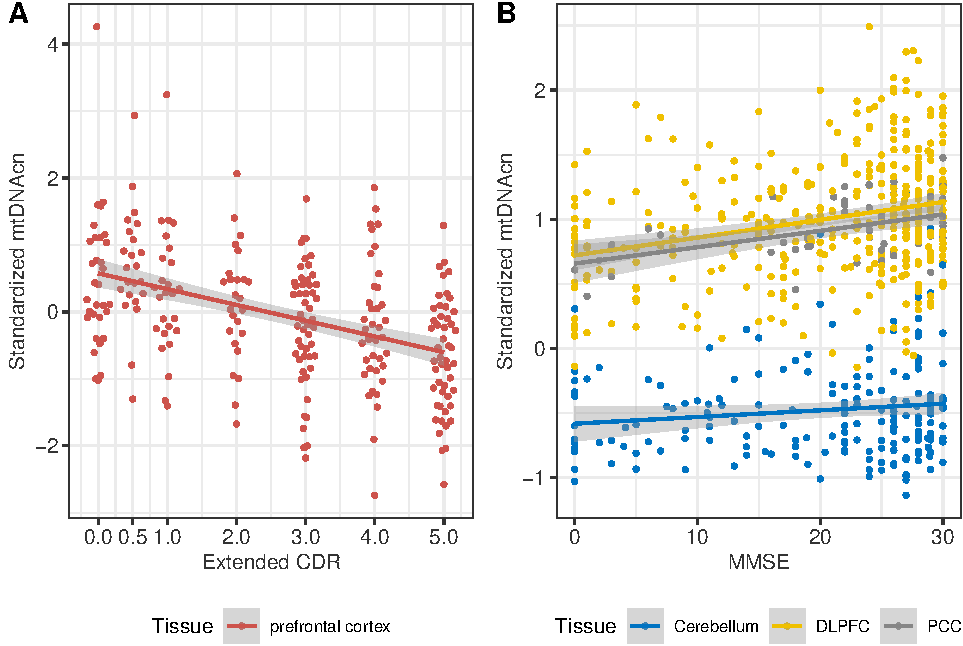
\includegraphics{notebook_files/figure-latex/print-aaic-plots-1.pdf}
\caption{\label{fig:print-aaic-plots}Relationship between mtDNAcn and CDR \& MMSE in MSBB and ROSMAP}
\end{figure}

\label{tab:aaic-tab-cdr}Assocation of mtDNA with CDR in MSBB

term

estimate

std.error

statistic

p.value

(Intercept)

1.859

1.037

1.793

0.074

z\_mtdnacn

-0.705

0.097

-7.301

3.41e-12

aod

0.002

0.012

0.192

0.848

sexM

0.084

0.215

0.388

0.698

apoe4e4+

0.724

0.200

3.621

3.52e-04

Haplogroup

macroI

0.938

0.918

1.022

0.308

macroJ

0.866

0.308

2.809

0.005

macroK

0.087

0.255

0.343

0.732

macroT

0.818

0.398

2.055

0.041

macroU

0.470

0.361

1.302

0.194

macroV

0.748

0.395

1.896

0.059

macroW

0.801

0.916

0.874

0.383

macroX

-0.769

0.794

-0.968

0.334

\label{tab:aaic-tab-mmse}Assocation of mtDNA with MMSE in ROSMAP

term

estimate

std.error

statistic

p.value

(Intercept)

49.199

4.450

11.056

2.19e-26

z\_mtdnacn

4.017

0.748

5.368

1.07e-07

age\_death

-0.281

0.049

-5.744

1.36e-08

msexM

0.823

0.674

1.222

0.222

apoe4e4+

-4.529

0.727

-6.230

7.89e-10

studyROS

-1.110

0.644

-1.722

0.085

Tissue

Source.Tissue.TypeDLPFC

-5.443

1.310

-4.156

3.62e-05

Source.Tissue.TypePCC

-3.561

1.604

-2.220

0.027

Haplogroup

macroI

1.062

1.737

0.611

0.541

macroJ

-0.959

1.181

-0.812

0.417

macroK

-1.863

1.241

-1.502

0.134

macroT

-0.033

1.089

-0.031

0.976

macroU

-1.209

0.919

-1.316

0.188

macroV

-1.873

1.479

-1.267

0.206

macroW

-5.087

2.514

-2.023

0.043

macroX

2.000

2.629

0.761

0.447

\textbf{Conclusion:} Mitochondrial dysfunction as measured by mtDNA-CN is associated with worse cognitive performance, suggesting that mitochondrial function plays a role in the pathogenesis of Alzheimer's Disease. However, further research is needed to determine if mitochondrial dysfunction causes, mediates, or is a by-product of AD pathogenesis, in particular whether neuronal loss is an unobserved confounder that could be driving the observed associations.

\hypertarget{final-words}{%
\chapter{Final Words}\label{final-words}}

We have finished a nice book.

\bibliography{book.bib,packages.bib}

\end{document}
